\chapter{Subjective Timbre Evaluation}
\label{chap:TimbreEvaluation}
	\todo{Come up with a better name for this chapter.}

\section{Introduction}
\label{sec:TimbreEvaluation-Introduction}
	In order to manipulate the perceptual characteristics of a sound it is necessary to know the relationships between
	low level audio features and semantic descriptions. In Chapter \ref{chap:Timbre} several different methods for
	obtaining this information were discussed.  In this chapter a new method of collecting semantically annotated audio
	feature data is presented (Section \ref{sec:TimbreEvaluation-DAWBasedTimbreEvaluation}). Data gathered using this
	method is then analysed, producing a list of semantic descriptors and the low level audio features which contribute
	to them (Section \ref{sec:TimbreEvaluation-Analysis}).

\section{Production Environment Timbre Evaluation} % this name will probably change
\label{sec:TimbreEvaluation-DAWBasedTimbreEvaluation}
	The perceptual listening test methodologies discussed in Section \ref{sec:Timbre-ListeningTests} rely on the
	participants performing a certain set of tasks. While this structure helps to reduce the number of variables in an
	experiment, it does not necessarily reflect the way audio is treated in a production environment.

	A new methodology has been developed in which the analysis of timbre is introduced into a typical music production
	workflow, causing minimal interruption to the producer. This methodology aims to answer the question "What terms do
	music producers use to describe the timbral transforms they apply to audio during the creation of music?". 

	This section will detail a typical production workflow is and how semantic information can be gathered.

	\subsection{Music Production Workflow}
	\label{sec:TimbreEvaluation-DAWBasedTimbreEvaluation-Workflow}
		A full discussion of the music production process is given by \citet{dittmar2013audio}. In brief the
		production workflow is spilt into four main stages:

		\begin{itemize}
			\item Recording
			\item Editing
			\item Mixing
			\item Mastering
		\end{itemize}

		At every stage of this process, semantic descriptors are often used to communicate the desired timbral
		qualities of the audio. For instance, one my ask that a certain microphone be used because of the `warmth'
		it adds to the recorded sound. During the mixing and mastering stages, audio processing effects are applied
		to shape the timbre further. These stages will be the focus of this section as the aim of this thesis is
		to improve the intuitiveness of these effects.

		Historically, audio production required the use of several pieces of electronic hardware, including
		microphones, a mixing console, audio processing effects and a recording device. Modern music production
		techniques utilise Digital Audio Workstation (DAW) software. This software performs the tasks of many
		pieces of hardware, enabling users to record, edit and mix multiple tracks of audio using a computer. 
		
	\subsection{Analysis of Timbre Inside the DAW}
	\label{sec:TimbreEvaluation-DAWBasedTimbreEvaluation-InDAW}
		An ideal way to collect timbral information during music production would be to have the DAW analyse the
		audio tracks used and production techniques applied. Information which could be gathered directly from the
		DAW, with no extra input from the user, includes:

		\begin{itemize}
			\item Information about the audio processing chain:
			\begin{itemize}
				\item The effects applied to each track.
				\item The order in which these effects are applied.
				\item The parameter settings of these effects.
			\end{itemize}
			\item Features of the audio signal at every stage in the processing chain.
		\end{itemize}

		Additional information can be gathered by prompting the user for input:

		\begin{itemize}
			\item The genre of music being produced.
			\item The content of the separate audio tracks (what instruments etc.).
			\item Semantic terms which describe the timbral transforms applied by each audio
			      effect.
		\end{itemize}

		Achieving this would require the creation of a new DAW, which would be impractical for the current
		research. DAWs are comprehensive software packages which perform many more tasks than the application of
		audio effects (project management, audio editing functionality etc.). A lot of effort would be expended in
		implementing these features before any timbral data could be collected. Music producers also tend to have a
		preferred DAW with which they work most fluidly. Convincing producers to use a new DAW for the purposes of
		research would be a difficult task.

		Third party developers can produce extensions to DAWs known as plug-ins. Plug-Ins provide additional audio
		processing functionality to the DAW environment. They can optionally expose their own parameters which
		users can adjust to achieve their desired effect. There are several different formats in which audio
		plug-ins can be distributed (VST, AU etc.). Most of the commonly used DAWs support plug-ins in one or more
		of these formats.

		Audio plug-ins provide a good platform to allow producers to provide semantic terms and audio feature
		information from within their preferred DAW. As part of this research a suite of audio plug-ins which
		extract this information have been developed. They have been released under the title Semantic Audio
		Feature Extraction (SAFE) Plug-Ins \footnote{The most recent versions of the SAFE plug-ins can be
		downloaded from \href{http://www.semanticaudio.co.uk/projects/download/}
		{www.semanticaudio.co.uk/projects/download}.}.

	\subsection{SAFE Plug-Ins}
	\label{sec:TimbreEvaluation-DAWBasedTimbreEvaluation-SAFE}
		The SAFE plug-ins consist of four commonly used audio effects: Equaliser, Distortion, Compressor and
		Reverb. As part of the plug-ins's interface, the user has the option to save a semantic description of the
		application of the effect. The interface for the SAFE Distortion is shown in Figure
		\ref{fig:SAFE-Distortion}. Upon saving a description the plug-in will record and analyse five seconds of
		audio at its inputs and outputs. When the analysis is completed the results are stored, containing:

		\begin{itemize}
			\item The users semantic description of the effect's application.
			\item The plug-in's current parameter settings.
			\item The features of the audio before and after processing.
			\item Some additional data about the user and the track being worked on.
			\begin{itemize}
				\item The genre.
				\item The instrument.
				\item The users age.
				\item The users location.
				\item The users primary language.
				\item The number of years experience the user has in music production.
			\end{itemize}
		\end{itemize}

		\begin{figure}[h!]
			\centering
			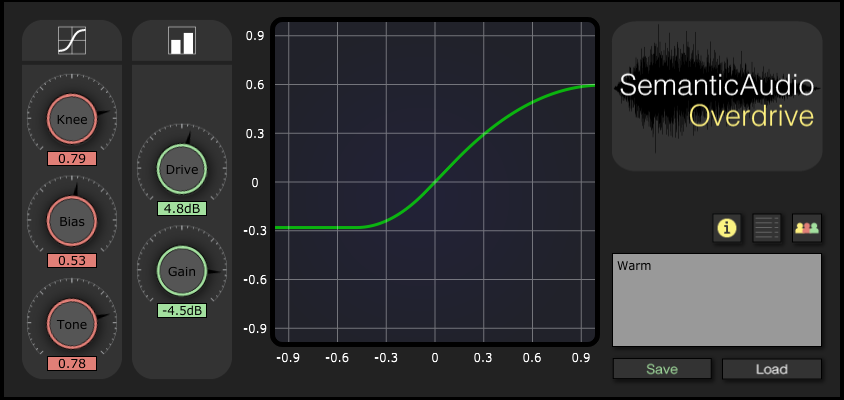
\includegraphics[width=0.8\textwidth]{chapter4/Images/SAFEDistortion.png}
			\caption{The interface for the SAFE distortion plug-in.}
			\label{fig:SAFE-Distortion}
		\end{figure}

		The audio is analysed in frames of 4096 samples using the LibXtract software library
		\citep{bullock2007libxtract}, calculating 80 different audio features for each frame. These features are
		split into five groups as follows:

		\begin{itemize}
			\item {\bf{Temporal Features:}} Features calculated from the temporal representation of the signal.
			\begin{itemize}
				\item Signal Mean ($\mu$), Signal Variance ($\sigma^{2}$), Signal Standard Deviation
				      ($\sigma$), RMS Amplitude ($\textrm{RMS}$) and Zero Crossing Rate ($\textrm{ZCR}$).
			\end{itemize}
			\item {\bf{Spectral Features:}} Features calculated from the DFT of the signal.
			\begin{itemize}
				\item Spectral Centroid ($\mu_{\textrm{s}}$), Spectral Spread ($\sigma_{\textrm{s}}^{2}$),
				      Spectral Standard Deviation ($\sigma_{\textrm{s}}^{2}$), Spectral Skewness
				      ($\gamma_{\textrm{s}}$), Spectral Kurtosis ($\kappa_{\textrm{s}}$), Jensen
				      Irregularity ($\textrm{JI}$), Krimphoff Irregularity ($\textrm{KI}$), $f_{0}$,
				      Spectral Smoothness ($\textrm{SSm}$), Spectral Roll Off ($\textrm{SRO}$), Spectral
				      Flatness ($\textrm{SF}$), Tonality ($\tau$), Spectral Crest ($\textrm{SC}$)
				      and Spectral Slope ($\textrm{SSl}$).
			\end{itemize}
			\item {\bf{Peak Spectral Features:}} Features calculated from the spectral partials of the signal.
			\begin{itemize}
				\item Peak Spectral Centroid ($\mu_{\textrm{p}}$), Peak Spectral Spread
				      ($\sigma_{\textrm{p}}^{2}$), Peak Spectral Standard Deviation
				      ($\sigma_{\textrm{p}}^{2}$), Peak Spectral Skewness ($\gamma_{\textrm{p}}$), Peak
				      Spectral Kurtosis ($\kappa_{\textrm{p}}$), Peak Jensen Irregularity
				      ($\textrm{JI}_{\textrm{p}}$), Peak Krimphoff Irregularity
				      ($\textrm{KI}_{\textrm{p}}$), Peak Tristimuli ($T_{\textrm{p}1}$, $T_{\textrm{p}2}$
				      and $T_{\textrm{p}3}$) and Inharmonicity ($I$).
			\end{itemize}
			\item {\bf{Harmonic Spectral Features:}} Features calculated from the harmonic partials of the
			      signal.
			\begin{itemize}
				\item Harmonic Spectral Centroid ($\mu_{\textrm{h}}$), Harmonic Spectral Spread
				      ($\sigma_{\textrm{h}}^{2}$), Harmonic Spectral Standard Deviation
				      ($\sigma_{\textrm{h}}$), Harmonic Spectral Skewness ($\gamma_{\textrm{h}}$), Harmonic
				      Spectral Kurtosis ($\kappa_{\textrm{h}}$), Harmonic Jensen Irregularity
				      ($\textrm{JI}_{\textrm{h}}$), Harmonic Krimphoff Irregularity
				      ($\textrm{KI}_{\textrm{h}}$), Tristimuli ($T_{1}$, $T_{2}$ and $T_{3}$), Noisiness
				      ($N$) and Odd to Even Harmonic Ratio ($\textrm{ROE}$).
			\end{itemize}
			\item {\bf{Bark Coefficients (}}$\textrm{Bark}_{0\textrm{-}24}${\bf{):}} The 25 bark band
			      coefficients.
			\item {\bf{MFCCs (}}$\textrm{MFCC}_{0\textrm{-}12}${\bf{):}} The 13 MFCCs.
		\end{itemize}

		One disadvantage in using plug-ins is that they cannot gather information about the processing chain they
		may be a part of. The timbral transform the user is describing may be the result of several effects working
		together. This can be mitigated somewhat by asking users to describe only the effect the plug-in in
		question is providing.

		The SAFE plug-ins suffer from the same issues other distributed tests do. The researcher forfeits control
		over the listening environment in order to gather results from a much larger sample of people. In fact they
		provide even lest control than methodologies like that used in the Social EQ project
		\citep{cartwright2013socialeq} in that the choice of audio samples being used is decided by the test
		subject. This control is relinquished in order to access a greater user base. The metadata fields allow the
		collected data to be categorised if information about a particular genre or instrument is desired.

		\note{Probably explain the need to use an ontology, something about being machine navigable or something.}

	\subsection{SAFE Ontology}
	\label{sec:TimbreEvaluation-DAWBasedTimbreEvaluation-SAFEOntology}
		The data collected using the SAFE plug-ins is stored as RDF triples using the SAFE ontology.  The SAFE
		Ontology was designed to describe the semantics relating to the application of an audio effect and the
		audio features of the signals involved. It acts as an extension to the Audio Effects Ontology
		\citep{wilmering2013the}, introducing additional concepts for the description of semantic data.  This
		additional data can be separated into three groups:

		\begin{itemize}
			\item Metadata describing the application of the effect.
			\item Audio feature data for the input and output signals.
			\item Provenance of the data.
		\end{itemize}

		Each entry in the SAFE dataset is described using the \emph{studio:Transform} concept, applying some
		semantic transform to a set of input signals to produce a set of output signals. The structure of this data
		is shown in Figure \ref{fig:TransformGraph}.

		\begin{figure}[h!]
			\centering
			\begin{tikzpicture}[->,>=stealth',node distance=3cm]
				\tikzstyle{object} = [style=ellipse]

				\node[object, fill=blue] (transform) {studio:Transform};
				\node[object, fill=green] (signal) [below left of=transform] {mo:Signal};
				\node[object, fill=orange] (descriptor) [above of=transform] {safe:DescriptorItem};
				\node[object, fill=orange] (metadata) [below right of=transform] {safe:MetadataItem};
				\node[object, fill=pink] (device) [above right=1.5cm and 0.8cm of transform] {afx:Device};
				\node[object, fill=pink] (state) [above left=1.5cm and 0.8cm of transform] {afx:State};
				\node[object, fill=gray] (harsh) [above=1cm of descriptor] {"Harsh"};

				\path (transform) edge [bend left] node [right, overlay] {prov:used} (signal)
				      edge [bend right] node [left, overlay] {prov:generated} (signal)
				      edge node [right, overlay] {safe:descriptor} (descriptor)
				      edge [bend left] node [right, overlay] {safe:metadata} (metadata)
				      edge [bend right] node [right, overlay] {studio:effect} (device)
				      edge [bend left] node [left, overlay] {afx:state} (state)
				      (signal) edge [bend right] node [below, overlay] {safe:metadata} (metadata)
				      (descriptor) edge node [right, overlay] {rdfs:comment} (harsh);
			\end{tikzpicture}
			\caption{The structure used to describe the application of an audio effect.}
			\label{fig:TransformGraph}
		\end{figure}

		Here, users provide a term, or series of terms, to describe the transform applied by the audio effect in
		its current state. This should describe the perceived difference between the output and input signals. In
		the SAFE Ontology this is modelled through the \emph{safe:DescriptorItem} concept which provides a semantic
		description for each transform. Metadata items are used to provide details about the application domain of
		the effect, where each metadata item describes one property of an object, the property being identified
		using an \emph{rdfs:label} and the description provided using an \emph{rdfs:comment}. Each object described
		by a metadata item has its own set of properties, ``genre'' and ``instrument'' metadata tags, for example,
		describe an audio signal, while ``location'' metadata tags describe a transform.

		The analysis of audio signals is described using the concept \emph{safe:FeatureExtractionTransform},
		similar to a \emph{studio:Transform} but taking an audio signal as input and producing a time series of
		feature values at the output, as shown in Figure \ref{fig:ExtractionGraph}.

		\begin{figure}[h!]
			\centering
			\begin{tikzpicture}[->,>=stealth',node distance=3cm]
				\tikzstyle{object} = [style=ellipse]

				\node[object, fill=orange] (extraction) {safe:FeatureExtractionTransform};
				\node[object, fill=gray] (feature) [above of=extraction] {"Spectral Centroid"};
				\node[object, fill=gray] (frameSize) [above left of=extraction] {"4096"};
				\node[object, fill=gray] (stepSize) [above right of=extraction] {"1024"};
				\node[object, fill=green] (signal) [below left of=extraction] {mo:Signal};
				\node[object, fill=purple] (event) [below right of=extraction] {event:Event};
				\node[object, fill=yellow] (interval) [below=1cm of signal] {tl:Interval};
				\node[object, fill=yellow] (instant) [below=1cm of event] {tl:Instant};
				\node[object, fill=yellow] (timeline) [below right of=interval] {tl:TimeLine};
				\node[object, fill=gray] (value) [below right=0.2cm and 0.6cm of event] {"2543.4"};
				\node[object, fill=gray] (time) [below right=0.2cm and 0.6cm of instant] {"4048"};

				\path (extraction) edge [bend left] node [left, overlay] {safe:frameSize} (frameSize)
				      edge [bend right] node [right, overlay] {safe:stepSize} (stepSize)
				      edge node [right, overlay] {rdfs:label} (feature)
				      edge [bend right] node [left, overlay] {prov:used} (signal)
				      (signal) edge node [left, overlay] {mo:time} (interval)
				      (event) edge node [left, overlay] {event:time} (instant)
				      edge [bend right] node [right, overlay] {prov:wasGeneratedBy} (extraction)
				      edge node [above right, overlay] {af:feature} (value)
				      (interval) edge [bend right] node [left, overlay] {tl:onTimeLine} (timeline)
				      (instant) edge [bend left] node [right, overlay] {tl:onTimeLine} (timeline)
				      edge node [above right, overlay] {tl:at} (time);

			\end{tikzpicture}
			\caption{The structure used to describe the features of an audio signal.}
			\label{fig:ExtractionGraph}
		\end{figure}

		Here, The SAFE Ontology makes extensive use of the Provenance Ontology to identify the origins of the data.
		Each element of data constitutes a \emph{prov:Entity} which was generated by a \emph{prov:Activity}. These
		\emph{prov:Activity} nodes are in turn associated with a \emph{prov:Agent} identifying the way that the
		data was produced.

		When using the SAFE plug-ins, users are required to provide a descriptor for a transform, meaning that
		every \emph{safe:DescriptorItem} node in the dataset is attributed to a particular user. Conversely, the
		metadata fields are not mandatory. In situations where a user has not filled in certain metadata fields
		their values can be predicted on the server using supervised machine learning. Using the Provenance
		Ontology, each metadata entity can be attributed to a particular agent, allowing it to be understood as
		human or machine labelled. This allows queries on the dataset to request only the more reliable
		user-labeled data or, for example, compare data produced using different classification algorithms.

		The Provenance Ontology is also used to describe the algorithms which produce audio feature data. Each
		\emph{safe:FeatureExtractionTransform} node is a \emph{prov:Activity} which can be associated with a
		particular implementation of the algorithm it uses (e.g. the LibXtract \citep{bullock2007libxtract}
		spectral centroid function). Say a discrepancy was found between two implementations of a given feature
		extraction algorithm, the provenance data allows queries to filter results to remove those generated using
		an earlier or incompatible implementation. Further use of provenance describes the role of a user in the
		application of a transform. Storage of this data allows the simple retrieval of all transforms associated
		with a particular user, allowing users to maintain personal libraries of semantic presets amongst the
		entire SAFE dataset.

\section{Analysis}
\label{sec:TimbreEvaluation-Analysis}
	In this section the data collected using the SAFE plug-ins is analysed. For the purposes of this study only the
	data from the distortion and equaliser plug-ins is used, as these effects best represent the timbral transforms
	which can be applied using harmonic excitation. The distortion demonstrating the effects of introducing new
	spectral content and the equaliser demonstrating the effects of manipulating the existing spectral content.

	Firstly, the terms used to describe transforms using each plug-in are investigated (Section
	\ref{sec:TimbreEvaluation-Analysis-TermUsage}). This provides insight into the language used to describe audio in
	the production environment, also showing what terms are shared across processing techniques and those which are
	reserved for particular effect. Secondly, clustering techniques are used in order to group these terms into groups
	which describe similar audio signals / transforms, finding terms which are synonymous when used to describe
	timbre (Section \ref{sec:TimbreEvaluation-Analysis-TermClustering}). Finally, timbre spaces are constructed using
	PCA in order to find the most salient audio features which contribute to the differences in timbral description.

	\subsection{Term Usage}
	\label{sec:TimbreEvaluation-Analysis-TermUsage}
		The dataset used for this work totals 304 transforms saved using the SAFE Distortion and 1483 transforms
		saved using the SAFE Equaliser. Several of the terms which describe these transforms are derived from the
		same root word, with the addition of suffixes such as `y' or `er' (e.g. `crunch' and `crunchy' or `bright'
		and `brighter'). It is assumed that the addition of such suffixes has no effect over how a term is used to
		describe timbre. As such, a stemming algorithm \citep{porter1980an} is used in order to reduce all
		descriptors in the dataset to their root words.  Additional processing is required after stemming so that
		all descriptors with the same root can be combined.  The Porter stemming algorithm replaces the letter y at
		the end of a word with the letter i, for this analysis these tailing i's are removed so that terms such as
		`fuzz' and `fuzzy' are reduced to the same root. In some cases the output must be further reduced, for
		example the term `muddy' is reduced to `mudd' which must have the tailing d removed to give the correct
		root `mud'.

		Tables \ref{tab:DistortionTerms} and \ref{tab:EqualiserTerms} show the terms most frequently used to
		describe transforms applied by the distortion and equaliser respectively. The frequency of each term
		indicates how many transforms it is used to describe. In some cases multiple descriptors are used to
		describe a transform. The numbers of transforms which share certain combinations of descriptors are shown
		in Tables \ref{tab:DistortionTermCombinations} and \ref{tab:EqualiserTermCombinations}. In total 85 of the
		distortion transforms are described by the 8 most popular distortion terms and 947 equaliser transforms are
		described by the 12 most popular equaliser descriptors.

		\begin{table}[h!]
			\centering
			\begin{tabular}{|c|c|}
				\hline
				\bf{Term} & \bf{Frequency} \tabularnewline
				\hline
				\hline
				crunch & 29 \tabularnewline
				\hline
				warm & 25 \tabularnewline
				\hline
				fuzz & 16 \tabularnewline
				\hline
				cream & 6 \tabularnewline
				\hline
			\end{tabular}
			\qquad
			\begin{tabular}{|c|c|}
				\hline
				\bf{Term} & \bf{Frequency} \tabularnewline
				\hline
				\hline
				bright & 5 \tabularnewline
				\hline
				harsh & 4 \tabularnewline
				\hline
				rasp & 4 \tabularnewline
				\hline
				smooth & 3 \tabularnewline
				\hline
			\end{tabular}
			\caption{Most commonly used terms from the distortion.}
			\label{tab:DistortionTerms}
		\end{table}

		\begin{table}[h!]
			\centering
			\begin{tabular}{|c|c|}
				\hline
				\bf{Terms} & \bf{Frequency} \tabularnewline
				\hline
				\hline
				fuzz / warm & 2 \tabularnewline
				\hline
				cream / warm & 1 \tabularnewline
				\hline
				cream / warm / fuzz & 1 \tabularnewline
				\hline
				crunch / harsh & 1 \tabularnewline
				\hline
				crunch / warm & 1 \tabularnewline
				\hline
			\end{tabular}
			\caption{Combinations of terms from the distortion.}
			\label{tab:DistortionTermCombinations}
		\end{table}

		\begin{table}[h!]
			\centering
			\begin{tabular}{|c|c|}
				\hline
				\bf{Term} & \bf{Frequency} \tabularnewline
				\hline
				\hline
				warm & 439 \tabularnewline
				\hline
				bright & 422 \tabularnewline
				\hline
				clear & 18 \tabularnewline
				\hline
				air & 18 \tabularnewline
				\hline
			\end{tabular}
			\qquad
			\begin{tabular}{|c|c|}
				\hline
				\bf{Term} & \bf{Frequency} \tabularnewline
				\hline
				\hline
				thin & 13 \tabularnewline
				\hline
				full & 10 \tabularnewline
				\hline
				boom & 9 \tabularnewline
				\hline
				box & 8 \tabularnewline
				\hline
			\end{tabular}
			\qquad
			\begin{tabular}{|c|c|}
				\hline
				\bf{Term} & \bf{Frequency} \tabularnewline
				\hline
				\hline
				tin & 7 \tabularnewline
				\hline
				deep & 6 \tabularnewline
				\hline
				mud & 6 \tabularnewline
				\hline
				harsh & 4 \tabularnewline
				\hline
			\end{tabular}
			\caption{Most commonly used terms from the equaliser.}
			\label{tab:EqualiserTerms}
		\end{table}

		\begin{table}[h!]
			\centering
			\begin{tabular}{|c|c|}
				\hline
				\bf{Terms} & \bf{Frequency} \tabularnewline
				\hline
				\hline
				bright / clear & 3 \tabularnewline
				\hline
				bright / clear / tin & 2 \tabularnewline
				\hline
				air / bright & 2 \tabularnewline
				\hline
				air / clear & 1 \tabularnewline
				\hline
				bright / thin & 1 \tabularnewline
				\hline
				bright / warm & 1 \tabularnewline
				\hline
				deep / boom & 1 \tabularnewline
				\hline
			\end{tabular}
			\caption{Combinations of terms from the equaliser.}
			\label{tab:EqualiserTermCombinations}
		\end{table}

		The terms `warm' and `bright' have been used to describe transforms applied using both the distortion and
		the equaliser effects, suggesting that the timbral characteristics these terms describe can be manipulated
		using either effect. These terms have much a much greater frequency in the equaliser as the result of an
		experiment in which participants were asked to use the equaliser to make audio samples `warmer' and
		`brighter' \citep{stasis2015a}. Other descriptors are only used to describe transforms applied using a
		specific effect, suggesting that a unique property of that effect produces that timbral result. For
		example, the term `crunch' is only used to in relation to the distortion effect.

	\subsection{Term Clustering}
	\label{sec:TimbreEvaluation-Analysis-TermClustering}
		Each of the terms arrived at, after stemming, in Section \ref{sec:TimbreEvaluation-Analysis-TermClustering}
		can be described by their position in a multi dimensional audio feature space. Each dimension of this space
		corresponds to one of the audio features extracted by the SAFE plug-ins. The position, $\mu_{d,k}$, of a
		term, $d$, in the $k$\super{th} dimension of the timbre space is calculated as the mean value of feature
		$k$ across every transform labelled with that descriptor (Equation \ref{eq:FeatureSpaceCoords}).

		\begin{equation}
			\mu_{d,k} = \frac{1}{N_{d}} \sum_{n = 1}^{N_{d}} \bar{x}_{d,n,k}
			\label{eq:FeatureSpaceCoords}
		\end{equation}

		Where $N_{d}$ is the number of transforms described by descriptor $d$, and $\bar{x}_{d,n,k}$ is the mean of
		feature $k$ across every frame of the signals analysed when saving the $n$\super{th} transform described by
		descriptor $d$.
		
		For each audio effect two separate feature spaces are constructed. In the first, a terms coordinates are
		calculated from the audio features of the processed signals. This gives insight into how terms are used to
		describe the absolute feature values of a signal (e.g. a signal with a spectral centroid between 4 and
		8kHz). In the second feature space, a terms coordinates are calculated from the difference between audio
		features of the output and input signals. This allows terms which describe the change of features
		associated with a transform (e.g. an increase in inharmonicity) to be identified.

		To identify groups of semantically similar descriptors, hierarchical clustering is applied to these feature
		spaces. Prior to clustering, each dimension of the feature space is standardised (i.e. scaled and offset
		such that is has a mean of zero and a standard deviation of one) to mitigate any effect the range of a
		particular audio feature might have on the clustering. Clusters are determined using the ward linkage
		criterion \citep{ward1963hierarchical} in order to minimise the variance within each cluster.

		\subsubsection*{Clustering of Distortion Terms}
			Figure \ref{fig:DistortionClusters} shows dendrograms illustrating the clustering of terms for the
			distortion features spaces. The clusters identified are similar for both the processed features
			(\ref{fig:DistortionProcessedClusters}) and the feature differences
			(\ref{fig:DistortionDifferenceClusters}), the cluster containing `harsh' and `bright' being the
			most distant from that containing `warm', `cream' and `fuzz' and the term `crunch' siting in a
			cluster separate from the majority of the other terms. This leads to the formation of three
			distinct timbral groups used to describe the application of distortion (`warm', `bright' and
			`crunch'). These clusters reflect some of the combinations of descriptors seen in Table
			\ref{tab:DistortionTermCombinations}, where `cream', `fuzz' and `warm' are often used alongside
			each other to describe a transform.

			\begin{figure}[h!]
				\centering
				\subfloat[Processed Features]
				{
					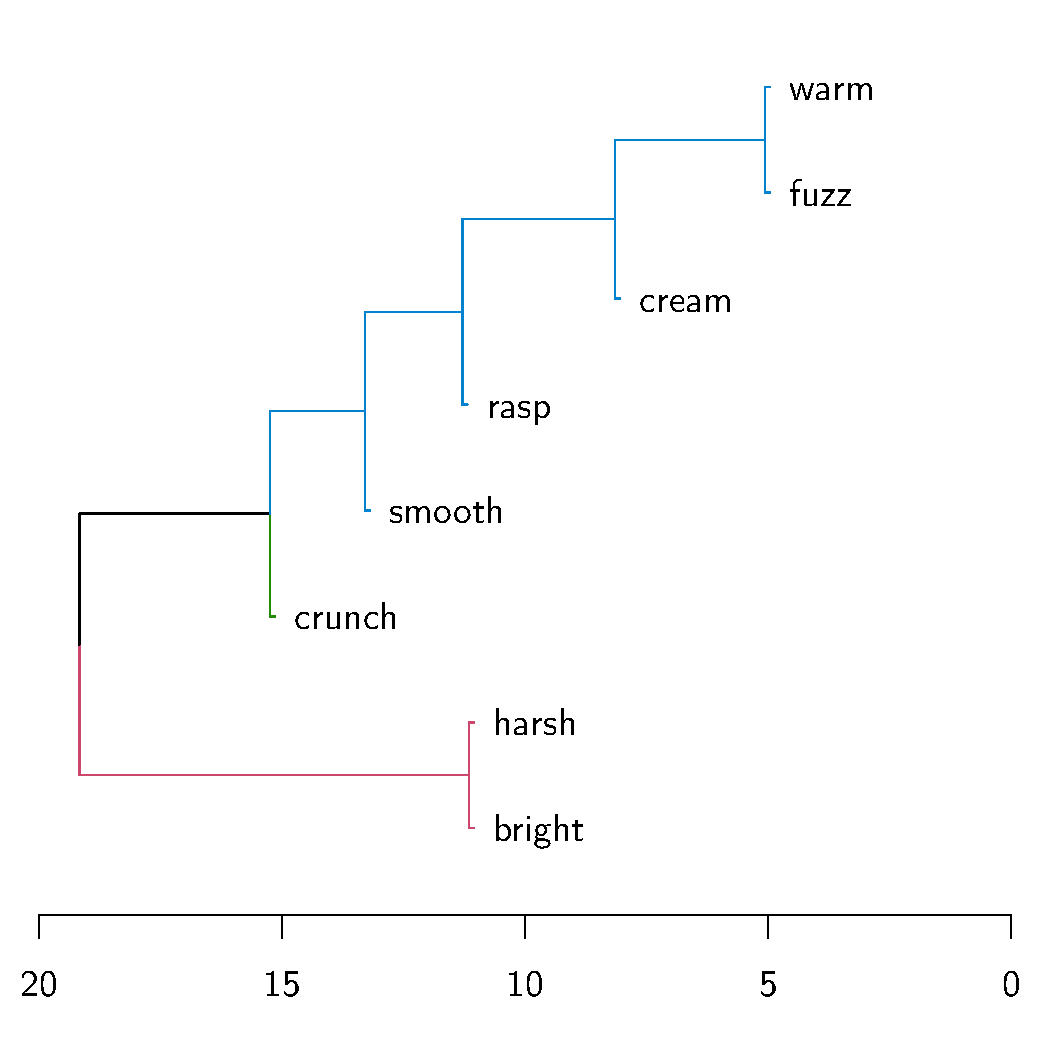
\includegraphics{chapter4/Images/DistortionProcessedClusters.pdf}
					\label{fig:DistortionProcessedClusters}
				}
				\subfloat[Feature Differences]
				{
					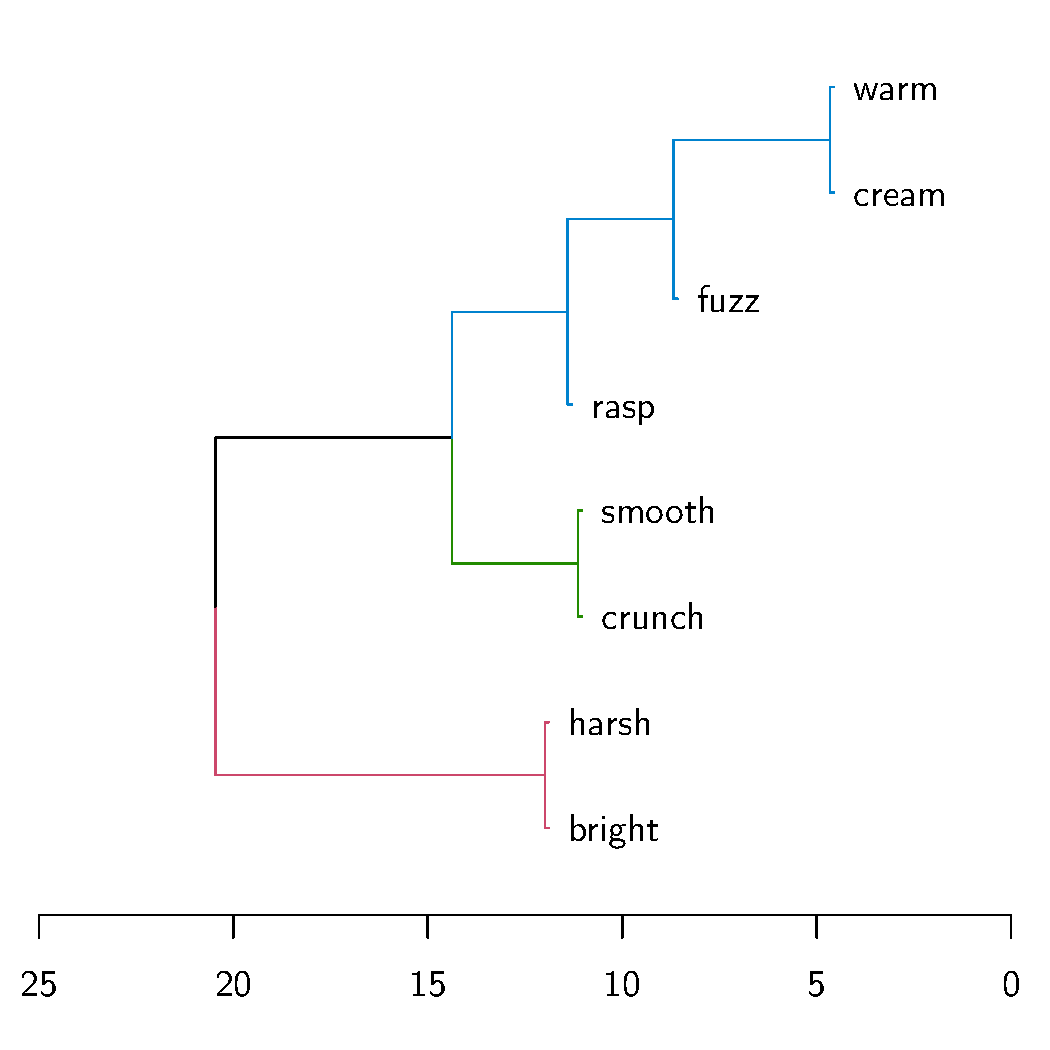
\includegraphics{chapter4/Images/DistortionDifferenceClusters.pdf}
					\label{fig:DistortionDifferenceClusters}
				}
				\caption{Clustering of descriptors from the distortion.}
				\label{fig:DistortionClusters}
			\end{figure}
		
		\subsubsection*{Clustering of Equaliser Terms}
			The clusters identified in the equaliser (Figure \ref{fig:EqualiserClusters}) show less agreement
			between the two different feature spaces. While the terms `warm' and `bright' were the most distant
			from each other in the distortion feature spaces, they are two of the closest terms in the
			equaliser's processed feature space (Figure \ref{fig:EqualiserProcessedClusters}). They are,
			however, separated well in the equaliser's feature difference space (Figure
			\ref{fig:EqualiserDifferenceClusters}) suggesting that the difference between these terms is better
			described by certain change in audio features rather than an absolute feature value.
			
			Within the equaliser's feature differences space, two main clusters are identified corresponding
			with the `warm' and `bright' clusters from the distortion feature spaces. The `warm' cluster
			includes the terms `deep' and `full', while the `bright' cluster includes the terms `tin', `thin',
			`clear' and `air'. An additional `mud' cluster, containing `mud', `boom' and `box', is also
			present. These three terms cluster better in the processed feature space indicating that they are
			more likely to describe a particular set of feature values rather than the properties of a
			transform. There is a similarity between these clusters and the combinations of descriptors used to
			describe equaliser transforms (Table \ref{tab:EqualiserTermCombinations}) suggesting that some of
			these terms may be synonymous with each other.

			\begin{figure}[h!]
%			This figure is da baddest figure, ask your dyslexic down syndromed mother.
				\centering
				\subfloat[Processed Features]
				{
					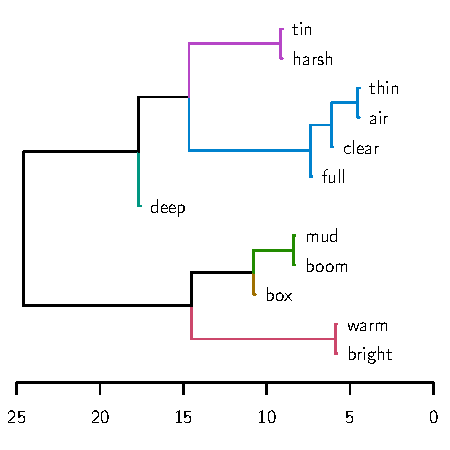
\includegraphics{chapter4/Images/EqualiserProcessedClusters.pdf}
					\label{fig:EqualiserProcessedClusters}
				}
				\subfloat[Feature Differences]
				{
					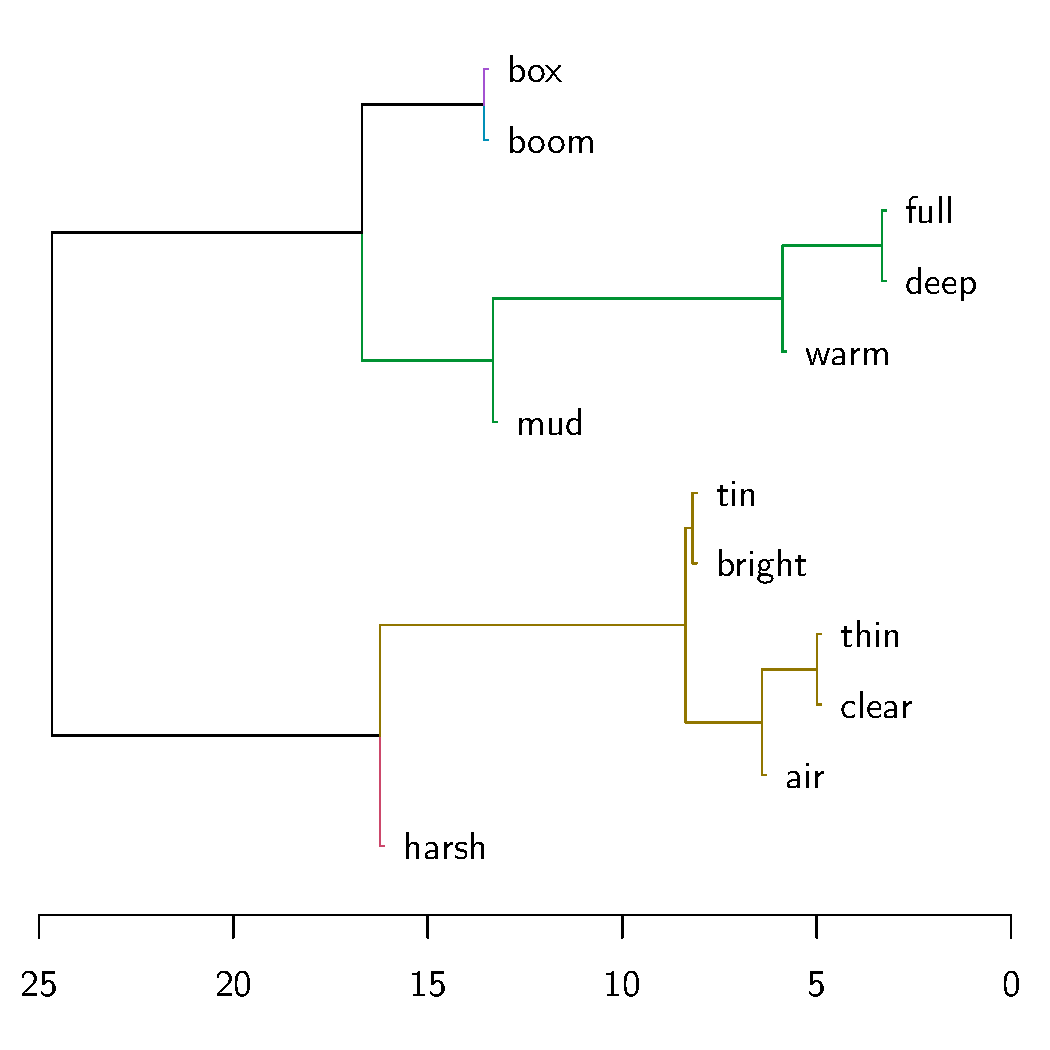
\includegraphics{chapter4/Images/EqualiserDifferenceClusters.pdf}
					\label{fig:EqualiserDifferenceClusters}
				}
				\caption{Clustering of descriptors from the equaliser.}
				\label{fig:EqualiserClusters}
			\end{figure}
		
		\subsubsection*{Clustering Across Both Effects}
			In order to investigate the similarity of descriptors across both plug-ins, their respective
			feature spaces are combined and clustering is applied to produce the dendrograms shown in Figure
			\ref{fig:CombinedClusters}. Descriptors are prepended with either and `E' or a `D' to distinguish
			between those describing distortion transforms and those describing equaliser transforms.

			\begin{figure}[h!]
				\centering
				\subfloat[Processed Features]
				{
					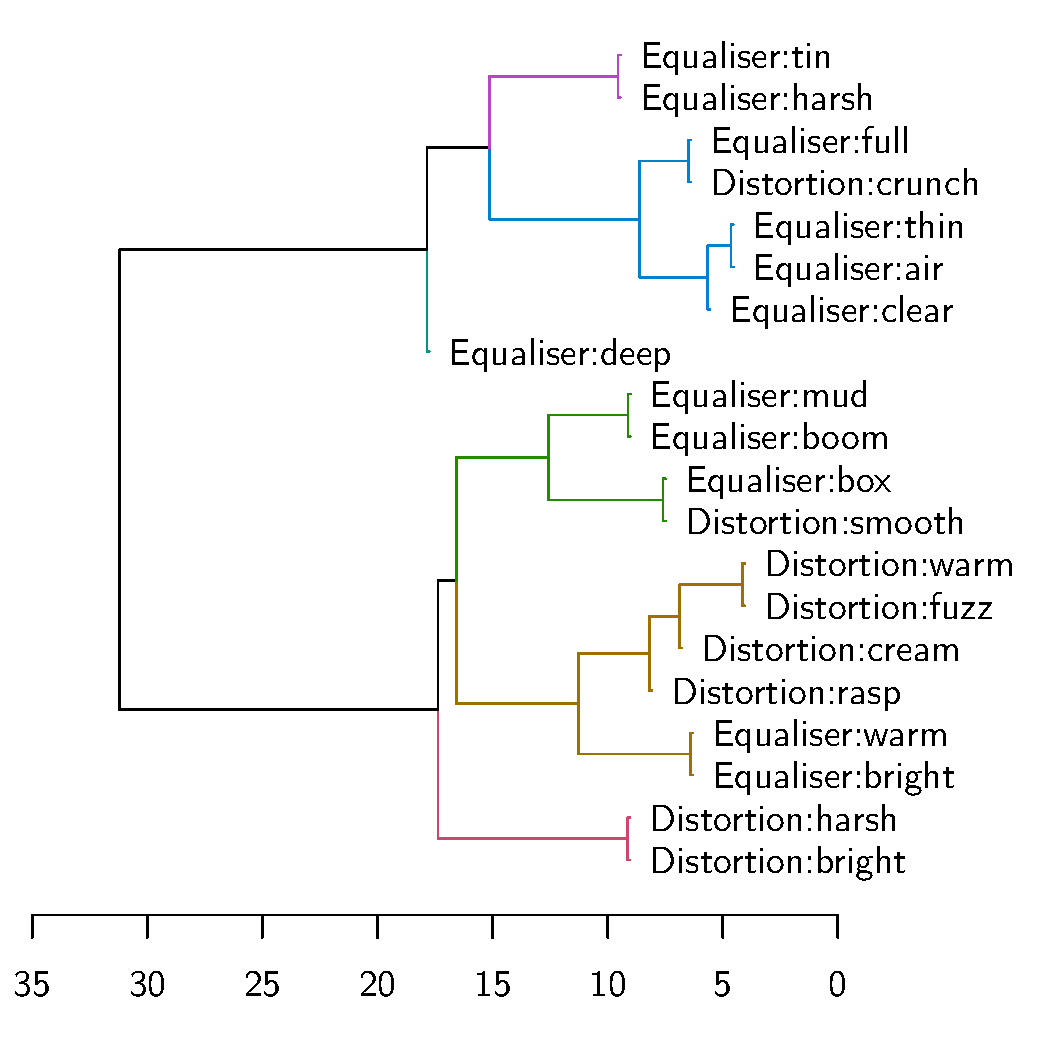
\includegraphics{chapter4/Images/CombinedProcessedClusters.pdf}
					\label{fig:CombinedProcessedClusters}
				}
				\subfloat[Feature Differences]
				{
					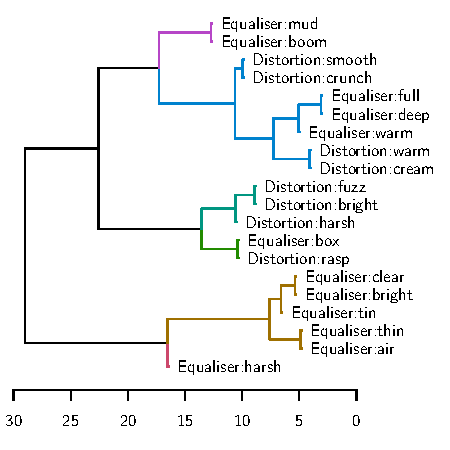
\includegraphics{chapter4/Images/CombinedDifferenceClusters.pdf}
					\label{fig:CombinedDifferenceClusters}
				}
				\caption{Clustering of descriptors from the both the distortion and equaliser.}
				\label{fig:CombinedClusters}
			\end{figure}

			Here the `warm' clusters from each plug-in's features spaces are combined, indicating that each of
			these descriptors describe similar transforms regardless of the processing method used. In contrast
			the `bright' groups remain separated into clusters comprised mostly of descriptors from a single
			plug-in, suggesting that the use of these terms may differ depending on the nature of the audio
			transform.  Further evidence of this is found in the similarity of the terms `bright' and `harsh'.
			When used to describe distortion transforms these terms always sit adjacent to one another in a
			cluster, whereas for equaliser transforms they are separated by a greater distance. These terms are
			more likely to be synonymous when describing audio processed by a distortion then they are for
			equalised audio. 

	\subsection{Agreement}
	\label{sec:TimbreEvaluation-Analysis-Agreement}
		The clustering performed in the previous section is applied to the mean positions of each of the terms. In
		reality a term describes several transforms which cover a region of the feature space. In order to draw
		conclusions about the region a descriptor covers in a feature space, it is necessary to have a measure of
		agreement for a descriptor. This measure describes the level to which different users agree on the semantic
		meaning of descriptive terms. The closer together the transforms, associated with a particular descriptor,
		are grouped in the feature space, the higher that descriptor's agreement score.

		\citet{cartwright2013socialeq} measure how well participants agree on the semantic annotation of graphic
		equaliser parameter settings. For each participant, a set of weightings is produced which describes the
		influence of each equaliser band on the perception of a particular timbral descriptor. The agreement score
		for a descriptor, $A(d)$, measures how similar these weightings are across different test participants
		using Equation \ref{eq:SocialEqAgreement}.

		\begin{equation}
			A(d) = \frac{\ln(N_{d})}{\sum_{k = 1}^{K} s_{d,k}^{2}}
			\label{eq:SocialEqAgreement}
		\end{equation}

		Where $N_{d}$ is the number of participants which have provided weightings for descriptor $d$,
		$s_{d,k}^{2}$ is the variance of weighting $k$ across those participants, and $K$ is the number of
		weightings in each set (i.e. the number of equaliser bands). The logarithm of the number of
		participants is used to account for Zipf's law, which states that the frequency with which a word is used
		is inversely proportional to its usage ranking (an integer describing the words popularity; 1 denoting the
		most commonly used word, 2 the second most common etc.) \citep{manning1999foundations}.

		This can be applied to data from the SAFE plug-ins by using audio feature values in place of parameter
		weightings. In Equation \ref{eq:SocialEqAgreement}, $N_{d}$ is then the number of transforms labelled with
		descriptor $d$, $s_{d,k}^{2}$ is the variance of feature $k$ across those transforms and $K$ is the total
		number of features. As when clustering, the feature space should be standardised prior to calculating
		agreement to remove the biasing effects caused by the ranges of each feature.

		This agreement score has several properties which do not necessarily reflect what is being measured:

		\begin{itemize}
			\item A larger number of transforms, $N_{d}$, produces higher agreement.
			\item It is assumed that high variance in any feature implies a disagreement. 
			\item It is assumed that all audio features are independent. 
			\item It is assumed that low variance in any feature implies an agreement. 
		\end{itemize}

		In this section an agreement measure which accounts for these points is developed.

		\subsubsection*{Number of Transforms}
			In Equation \ref{eq:SocialEqAgreement} the logarithm of the number of transforms, $N_{d}$, is used
			to scale the agreement score. This measures a different concept of agreement to what is desired for
			this work. It measures the size of a region in the feature space along with how many participants
			agree that the descriptor applies to the region, obscuring information about of how tightly the
			transforms in a region are clustered. A sufficiently large number of transforms will produce a
			large agreement score regardless of how spread apart they are. In this work, the agreement of
			participants as to the position of a descriptor in the feature space is needed. This is better
			measured by removing the scaling factor, giving Equation \ref{eq:ReciprocalOfSumAgreement}.

			\begin{equation}
				A(d) = \frac{1}{\sum_{k = 1}^{K} s_{d,k}^{2}}
				\label{eq:ReciprocalOfSumAgreement}
			\end{equation}

			Measuring agreement in this way provides an indication of how easily audio can be manipulated to
			exhibit a certain timbre. If the position of a descriptor in the feature space is well defined
			(occupies a small region) then the manipulations which need to be applied to the audio are better
			defined. The audio features of a signal must be moved to a particular location in the feature
			space. As the size of the region a descriptor occupies increases, the number of different
			manipulations which can be applied to a signal to place it within that region increases. The
			descriptor could describe various different timbral effects.

			To take account of the number of transforms labelled with a particular descriptor, Bessel's
			correction can be used in the calculation of variance as shown in Equation
			\ref{eq:UnbiasedVariance}. This uses the data available from a sample and uses it to approximate
			the variation present in the population.

			\begin{equation}
				s_{d,k}^{2} = \frac{1}{N_{d} - 1} \sum_{n = 1}^{N_{d}} (\bar{x}_{d,n,k} - \mu_{d,k})^{2}
				\label{eq:UnbiasedVariance}
			\end{equation}

			Where $\bar{x}_{d,n,k}$ and $\mu_{d,k}$ are as described for Equation \ref{eq:FeatureSpaceCoords}.

			Using this measure of variance in the agreement score provides an approximation of how closely
			clustered transforms, labeled with a certain descriptor, would be in a feature space which
			represents the whole population. In all further agreement score calculations it is assumed that the
			variances, or covariances, are measured using Bessel's correction.

		\subsubsection*{High Variance}
			A term exhibiting high variance in a particular audio feature could imply one of two things. Either
			that users do not agree on the position of the term in the feature space, or that that feature has
			no effect on the perception of the term. In the first case the agreement score should be decreased,
			but in the second the agreement score should not be affected. Because of this ambiguity, it is
			preferable that a high variance has negligible effect on the agreement score. In this way, if a
			high variance does imply disagreement it does not unduly increase the agreement score and if it
			does not imply disagreement it does to unduly decrease the agreement score.
			
			This can be implemented by changing Equation \ref{eq:ReciprocalOfSumAgreement} to be a sum of
			reciprocals rather than the reciprocal of a sum, as shown in Equation
			\ref{eq:SumOfReciprocalAgreement}.

			\begin{equation}
				A(d) = \sum_{k = 1}^{K} \frac{1}{s_{d,k}^{2}}
				\label{eq:SumOfReciprocalAgreement}
			\end{equation}

			Using this equation the agreement score is increased for each audio feature in which the
			descriptor exhibits a small variance, better identifying descriptors with a defined position in
			the feature space.

		\subsubsection*{Dependent Features}
			It may be the case that users agree that a particular term describes a relationship between several
			audio features (e.g. a spectral centroid lying at the 4\super{th} harmonic). Equations
			\ref{eq:SocialEqAgreement}, \ref{eq:ReciprocalOfSumAgreement} and \ref{eq:SumOfReciprocalAgreement}
			all ignore any dependence between audio features.

			Relationships between features can be taken into account by examining the covariance matrix,
			$\Sigma_{d}$, of the coordinates of the transforms associated with a descriptor, $d$. This is
			calculated using Equation \ref{eq:CovarianceMatrix}.

			\begin{equation}
				{\Sigma_{d}}_{ij} = \frac{1}{N_{d} - 1} \sum_{n = 1}^{N_{d}} 
						     (\bar{x}_{d,n,i} - \mu_{d,i})(\bar{x}_{d,n,j} - \mu_{d,j})
				\label{eq:CovarianceMatrix}
			\end{equation}
			
			The variances used in Equation \ref{eq:SumOfReciprocalAgreement} can then be substituted with the
			eigenvalues of this matrix, as shown in Equation \ref{eq:EigenvalueAgreement}.

			\begin{equation}
				A(d) = \sum_{k = 1}^{K} \frac{1}{\lambda_{d,k}}
				\label{eq:EigenvalueAgreement}
			\end{equation}
			
			Where $\lambda_{d, k}$ is the $k$\super{th} eigenvalue of the covariance matrix $\Sigma_{d}$.

			When using Equation \ref{eq:EigenvalueAgreement}, the number of eigenvalues used, $K$, needs to be
			carefully selected. If $N_{d}$ is less than or equal to the total number of audio features, the
			covariance matrix will be singular, meaning that one or more of its eigenvalues will be equal to
			zero. At most, only the $N_{d} - 1$ largest eigenvalues should be used.
			
			Any other eigenvalues equal to zero would imply a perfect linear relationship between a combination
			of audio features. If the features concerned are mathematically defined to be directly proportional
			then these zero eigenvalues should have no effect on the agreement score. If, however, a perfect
			linear relationship is discovered in the data, the agreement score should be increased
			accordingly. This raises an issue with Equation \ref{eq:EigenvalueAgreement} in that a devision by
			zero will occur if a perfectly linear relationship is discovered. This can be remedied by
			calculating the agreement using Equation \ref{eq:BoundedEigenvalueAgreement}. Calculating the
			agreement in this manner also has the advantage of bounding the agreement score between zero (no
			agreement) and $K$ (perfect agreement in all dimensions).

			\begin{equation}
				A(d) = \sum_{k = 1}^{K} \frac{1}{1 + \lambda_{d,k}}
				\label{eq:BoundedEigenvalueAgreement}
			\end{equation}

		\subsubsection*{Low Variance}
			Low variance in a particular audio feature does not necessarily imply an agreement between users.
			It may indicate a similarity between all of the audio segments processed, regardless of semantic
			labelling. To account for this, features which have low variance across the entire dataset can be
			disregarded. This can be achieved by calculating the agreement in a reduced dimensionality feature
			space.

			Using PCA, the dimensions with the largest variance in the feature space can be discovered. If the
			transforms labelled with a particular term exhibit a small variance in one of these dimensions it
			is likely that that term is well agreed upon. Agreement can be calculated in the PCA timbre space
			using Equation \ref{eq:BoundedEigenvalueAgreement}, with $\lambda_{d,k}$ being the $k$\super{th}
			eigenvalue of the covariance matrix of the principal components (PCs) for every transform labelled
			with descriptor $d$. As when calculating the agreement in the feature space, the coordinates of the
			transforms in each PC should be standardised to remove bias introduced by the proportions of total
			variance each PC describes.

			The number of PCs to use in the calculation of agreement is an important consideration. PCs which
			describe a low proportion of total variance should be discarded as is can not be known whether this
			low variance is due to user agreement. It is therefore recommended that a threshold is set, and
			only PCs which describe a proportion of variance above this threshold are used. Discarding the low
			variance PCs in this manner also removes any which have zero variance due to audio features
			which are defined to be directly proportional to one another, removing their effect on the
			agreement score.

			Further to this, the number of eigenvalues used, $K$, needs to be decided. Where $N_{d}$ is greater
			than the number of PCs used, all the eigenvalues should be used ($K$ equal to the number of PCs).
			For cases where $N_{d}$ is less than or equal to the number of PCs used, only $N_{d} - 1$
			eigenvalues should be used ($K = N_{d} - 1$). This dynamic value for $K$ has the benefit of
			reducing the agreement scores for terms which describe very few transforms. It also ensures that
			terms which describe only one transform will always receive an agreement score of zero, as $K$ will
			be equal to zero.

		\subsubsection*{Validation with Synthesised Data}
			To demonstrate the differences between Equations \ref{eq:SocialEqAgreement},
			\ref{eq:ReciprocalOfSumAgreement}, \ref{eq:SumOfReciprocalAgreement}, \ref{eq:EigenvalueAgreement}
			and \ref{eq:BoundedEigenvalueAgreement} artificial data can be synthesised which exhibits some of
			the issues discussed with Equation \ref{eq:SocialEqAgreement}.
			
			Figure \ref{fig:SynthesisedData} shows a synthesised, three dimensional, dataset containing four
			clusters of points. For ease of discussion it is assumed that this data represents the feature
			space after PCA has been applied. Each cluster has different properties which need to be taken into
			account when calculating the agreement score. Cluster 1 represents a set of points whose position
			in the PCA space is not agreed upon, exhibiting a high variance in every PC. Cluster 2 represents a
			set of points whose position is very well agreed upon, having low variance in every PC. Cluster 3
			represents a set of points whose position is only defined in one PC, having high variance in the
			other two. Cluster 4 represent a set of points which are defined by a relationship between two PCs,
			exhibiting high variance in all PCs but a strong correlation ($r = 0.9$) between PCs 1 and 2. The
			clusters were generated using the techniques discussed by \citet{ripley1987stochastic}, using the
			means, $\mu$, and covariance matrices, $\Sigma$, shown in Datum \ref{dat:ClusterStats}.

			\begin{datum}[h!]
				\centering
				\subfloat[Cluster 1]
				{
					\parbox{5cm}
					{
						\centering
						$\mu = \begin{bmatrix}
							     2 & 3 & 4
						       \end{bmatrix}$

						\vspace{1em}

						$\Sigma = \begin{bmatrix}
								5 & 0 & 0 \\
								0 & 5 & 0 \\
								0 & 0 & 5
							  \end{bmatrix}$
					}
					\label{dat:Cluster1Stats}
				}
				\qquad
				\subfloat[Cluster 2]
				{
					\parbox{5cm}
					{
						\centering
						$\mu = \begin{bmatrix}
							     4 & -2 & 1
						       \end{bmatrix}$

						\vspace{1em}

						$\Sigma = \begin{bmatrix}
								0.2 & 0 & 0 \\
								0 & 0.2 & 0 \\
								0 & 0 & 0.2
							  \end{bmatrix}$
					}
					\label{dat:Cluster2Stats}
				}

				\vspace{1.5em}

				\subfloat[Cluster 3]
				{
					\parbox{5cm}
					{
						\centering
						$\mu = \begin{bmatrix}
							     -2 & 0 & 2
						       \end{bmatrix}$

						\vspace{1em}

						$\Sigma = \begin{bmatrix}
								0.1 & 0 & 0 \\
								0 & 6 & 0 \\
								0 & 0 & 5
							  \end{bmatrix}$
					}
					\label{dat:Cluster3Stats}
				}
				\qquad
				\subfloat[Cluster 4]
				{
					\parbox{5cm}
					{
						\centering
						$\mu = \begin{bmatrix}
							     5 & -3 & 4
						       \end{bmatrix}$

						\vspace{1em}

						$\Sigma = \begin{bmatrix}
								5 & 0.9\sqrt{10} & 0 \\
								0.9\sqrt{10} & 2 & 0 \\
								0 & 0 & 4
							  \end{bmatrix}$
					}
					\label{dat:Cluster4Stats}
				}
				\caption{The means and covariance matrices for the clusters shown in Figure
					 \ref{fig:SynthesisedData}.}
				\label{dat:ClusterStats}
			\end{datum}

			\begin{figure}[h!]
				\centering
				\subfloat
				{
					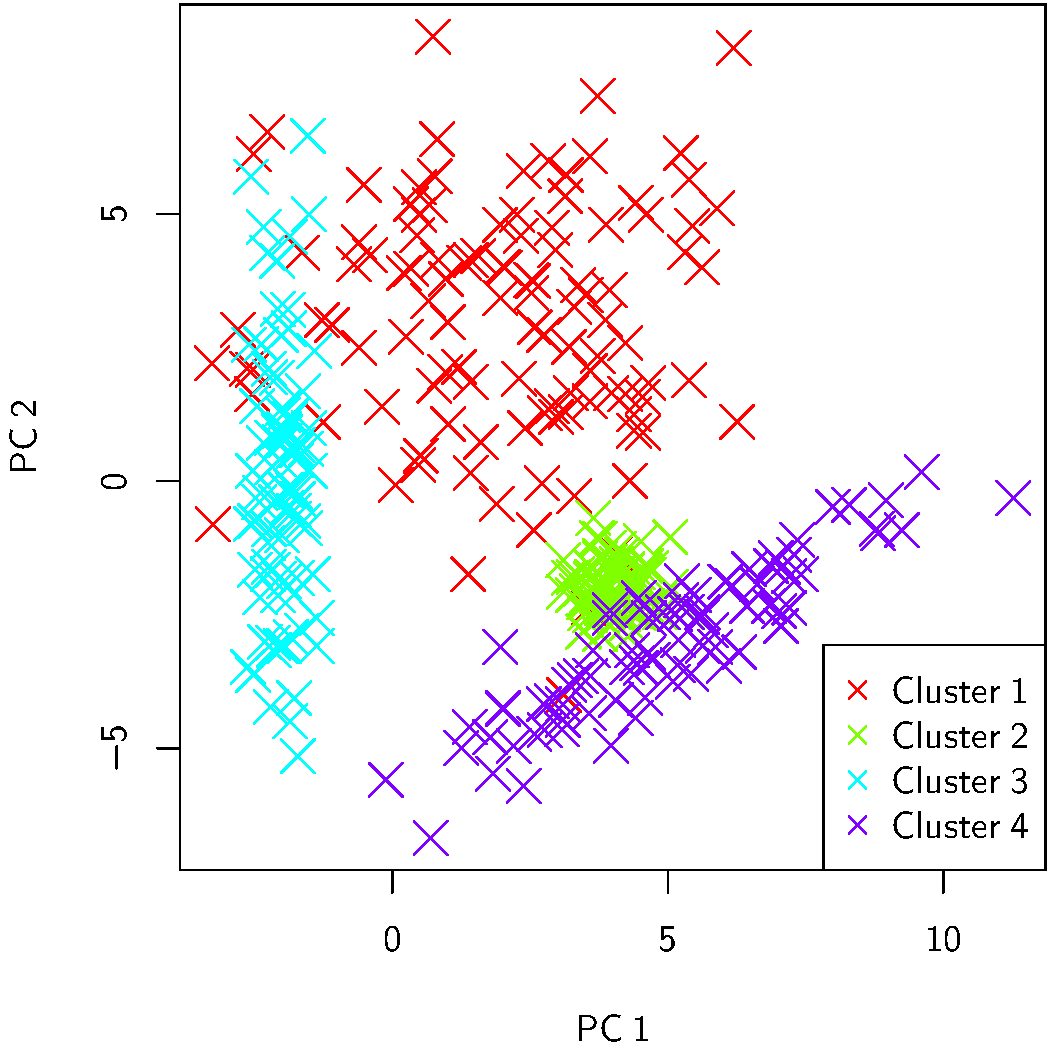
\includegraphics{chapter4/Images/ArtificialData1-2.pdf}
					\label{fig:EqualiserDifferencePCA}
				}
				\quad
				\subfloat
				{
					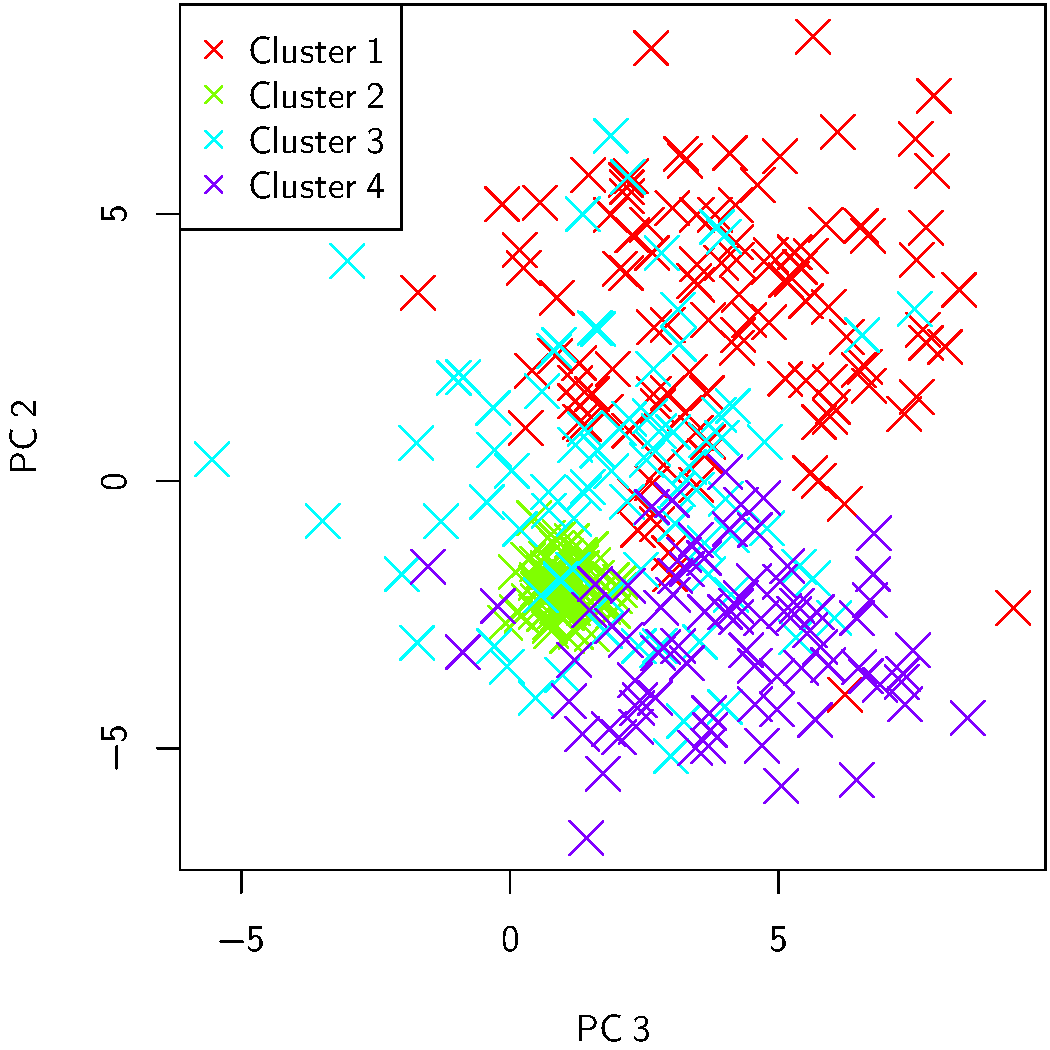
\includegraphics{chapter4/Images/ArtificialData3-2.pdf}
					\label{fig:EqualiserDifferenceCentroidsPCA}
				}
				\caption{Synthesised Data.}
				\label{fig:SynthesisedData}
			\end{figure}

			Visualising the data in Figure \ref{fig:SynthesisedData} provides intuition as to how an agreement
			score should rate each cluster. Cluster 1 should receive the lowest score as there is no
			discernible pattern to the data points. Cluster 2 should receive the highest score as it is very
			tightly clustered in all PCs. Both clusters 3 and 4 show some some patterns in the distribution.
			Cluster 3 has a well defined position in PC 1 while cluster 4 shows a strong relationship between
			PCs 1 and 2. The agreement scores for these clusters should reflect these patterns. Table
			\ref{tab:SynthesisedDataAgreement} shows agreement scores for the data shown in Figure
			\ref{fig:SynthesisedData}, calculated using Equations \ref{eq:SocialEqAgreement},
			\ref{eq:ReciprocalOfSumAgreement}, \ref{eq:SumOfReciprocalAgreement}, \ref{eq:EigenvalueAgreement}
			and \ref{eq:BoundedEigenvalueAgreement}.

			\begin{table}[h!]
				\centering
				\begin{tabular}{|c|c|c|c|c|c|}
					\cline{2-6}
					\multicolumn{1}{c|}{} & \multicolumn{5}{c|}{\bf{Agreement Score}} \tabularnewline
					\hline
					\bf{Cluster} & \bf{Equation \ref{eq:SocialEqAgreement}} & 
					\bf{Equation \ref{eq:ReciprocalOfSumAgreement}} &
					\bf{Equation \ref{eq:SumOfReciprocalAgreement}} & 
					\bf{Equation \ref{eq:EigenvalueAgreement}} &
					\bf{Equation \ref{eq:BoundedEigenvalueAgreement}} \tabularnewline
					\hline
					\hline
					\bf{1} & 2.3 & 0.5 & 4.7 & 4.7 & 1.8 \tabularnewline
					\hline
					\bf{2} & 55.1 & 12.2 & 117.9 & 117.9 & 2.9 \tabularnewline
					\hline
					\bf{3} & 2.7 & 0.6 & 95.7 & 95.7 & 2.1 \tabularnewline
					\hline
					\bf{4} & 2.9 & 0.7 & 7.7 & 34.8 & 2.1 \tabularnewline
					\hline
				\end{tabular}
				\caption{Agreement scores for the synthesised data.}
				\label{tab:SynthesisedDataAgreement}
			\end{table}

			The issues with Equations \ref{eq:SocialEqAgreement} and \ref{eq:ReciprocalOfSumAgreement} are
			immediately obvious. They ignore readily noticeable patterns in the data, giving clusters 1, 3 and
			4 similar agreement scores. By removing the assumption that high variance implies disagreement,
			Equation \ref{eq:SumOfReciprocalAgreement} takes account of the pattern in cluster 3. Equation
			\ref{eq:EigenvalueAgreement} removes the assumption that all PCs are independent enabling it to
			reflect the pattern shown in cluster 4. The final column of Table
			\ref{tab:SynthesisedDataAgreement} shows the bounding effect given by Equation
			\ref{eq:BoundedEigenvalueAgreement}.

	\subsection{Timbre Spaces}
	\label{sec:TimbreEvaluation-Analysis-TimbreSpaces}
		Clustering provides insight into the similarity of descriptive terms but does not show what properties of
		the signals / transforms contribute to the differences between descriptor clusters. Reducing the
		dimensionality of the audio feature space allows for the most salient audio features to be identified. To
		preserve as much of the audio feature data as possible, a different feature space, to that used for
		clustering, is constructed. Rather than each descriptor representing one point in the feature space, each
		individual transform represents its own point. 

		Two low dimensionality timbre spaces are generated for each effect, one from the feature space of the
		processed signals and the other from the feature space describing the difference in feature values between
		the processed and unprocessed signals. To generate these timbre spaces, the feature values from every
		applicable transform in the dataset (304 from the distortion and 1483 from the equaliser) are standardised
		and then undergo PCA. For every space, the knee of the PCA scree plot lies at five PCs. The final reduced
		dimensionality timbre spaces are then constructed from the first five PCs.

		These timbre spaces are analysed in various steps. Firstly the audio features which correlate most highly
		with each PC are determined. Features which satisfy a correlation criteria of $r > 0.7$ and $p < 0.01$ are
		deemed to be the salient features of each timbre space. Next the agreement scores for the relevant
		descriptors from Tables \ref{tab:DistortionTerms} and \ref{tab:EqualiserTerms} are calculated. As the
		timbre space is a product of PCA no additional PCA is needed, the high variance dimensions of the data have
		already been identified. Each timbre space is standardised and the covariance matrix for each descriptor is
		calculated. The agreement scores are then calculated from the eigenvalues of these covariance matrices
		using equation \ref{eq:BoundedEigenvalueAgreement} as discussed in Section
		\ref{sec:TimbreEvaluation-Analysis-Agreement}.
		
		Two types of graph are plotted to identify patterns within each timbre space. The first is a scatter plot
		in which the position of each individual transform is shown. These plots show the regions of the timbre
		space which have been described by each term. The second is a biplot showing the mean position of
		transforms labelled with each descriptor, along with vectors showing the influence of the most salient
		audio features in each PC. In these graphs the size of the text indicates the agreement score associated
		with that descriptor. In combination these two plots give a visual representation of how the audio features
		influence the use of descriptors.

		Additionally an impression of the spectral characteristics related to each descriptor can be seen by
		examining the bark band coefficients in the feature space. When applied to the processed feature space this
		provides a mean bark band spectrum of the output signals described with a particular term. When applied in
		the feature difference space it provides the mean spectral manipulation applied by transforms associated
		with a particular term.

		\subsubsection*{Distortion Processed Features}
			The first three PCs of the timbre space describing the processed signals produced by the distortion
			are shown in Figure \ref{fig:DistortionProcessedPCAs}. The corresponding agreement scores are shown
			in Table \ref{tab:DistortionProcessedAgreements}. The three terms with the highest agreement scores
			(`warm', `fuzz' and `crunch') are of particular interest.

			\begin{figure}[h!]
				\centering
				\subfloat
				{
					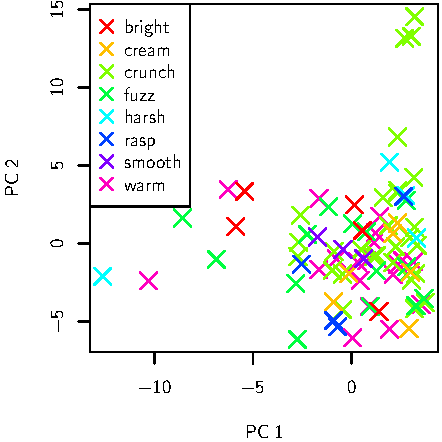
\includegraphics{chapter4/Images/DistortionProcessedPCA1-2.pdf}
					\label{fig:DistortionProcessedPCA1-2}
				}
				\quad
				\subfloat
				{
					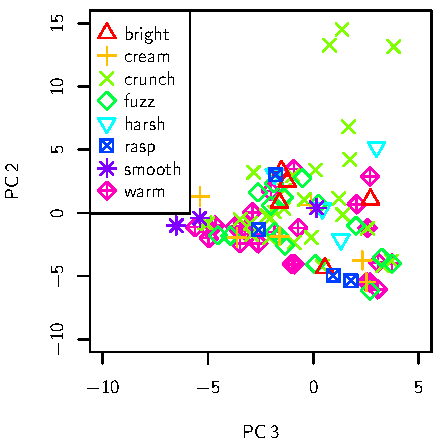
\includegraphics{chapter4/Images/DistortionProcessedPCA3-2.pdf}
					\label{fig:DistortionProcessedPCA3-2}
				}
				\caption{The distortion's processed feature timbre space.}
				\label{fig:DistortionProcessedPCAs}
			\end{figure}

			\begin{table}[h!]
				\centering
				\begin{tabular}{|c|c|}
	\hline
	\bf{Term} & \bf{Agreement} \tabularnewline
	\hline
	\hline
	warm & 0.71 \tabularnewline
	\hline
	fuzz & 0.57 \tabularnewline
	\hline
	crunch & 0.56 \tabularnewline
	\hline
	cream & 0.39 \tabularnewline
	\hline
\end{tabular}
\qquad
\begin{tabular}{|c|c|}
	\hline
	\bf{Term} & \bf{Agreement} \tabularnewline
	\hline
	\hline
	rasp & 0.32 \tabularnewline
	\hline
	bright & 0.20 \tabularnewline
	\hline
	harsh & 0.14 \tabularnewline
	\hline
	smooth & 0.07 \tabularnewline
	\hline
\end{tabular}

				\caption{The agreement scores for terms in the 
					 distortion's processed feature timbre space.}
				\label{tab:DistortionProcessedAgreements}
			\end{table}

			Referring back to the clusters shown in Figure \ref{fig:DistortionProcessedClusters}, `warm' and
			`fuzz' were found to be the most closely related descriptors in the distortion's processed feature
			space. This similarity is reflected in the Figure \ref{fig:DistortionProcessedPCAs} where the
			transforms labelled with these terms occupy similar regions of the timbre space. The third closest
			member of this cluster, `cream', can also bee seen to be distributed across the same region of the
			timbre space, further reinforcing the conclusion that these three terms are synonymous when used to
			describe signals processed by a distortion effect.

			This `warm' region is spread across the majority of the ranges of both PCs 1 and 3, while only
			occupying a lesser extent of the range of PC 2. In contrast, the region described by the term
			`crunch' is spread out across PCs 2 and 3 and concentrated to a smaller range of PC 1. This
			suggests that `warm', `fuzz' and `cream' are used to describe signals which lie somewhere between
			-5 and 5 in PC 2, while `crunch' is used to describe signals which line between -5 and 5 in PC 1.
			Signals which lie withing both of these ranges could potentially be described as both `warm' and
			`crunch'. Table \ref{tab:DistortionTermCombinations} confirms that one such combination of
			`warm' and `crunch' exists within the dataset.

			The salient features for this timbre space are shown in Datum
			\ref{dat:DistortionProcessedCorrelations}. The most salient in each PC are then visualised, along
			with the mean position and agreement score of each descriptor, in Figure
			\ref{fig:DistortionProcessedCentroidsPCAs}. 

			\begin{datum}[h!]
				\centering
				\begin{minipage}{0.9\textwidth}
					{\bf{PC 1:}} $\textrm{KI}$~($r~=~{-0.992}$), $\textrm{KI}_{\textrm{p}}$~($r~=~{-0.985}$), $\textrm{KI}_{\textrm{h}}$~($r~=~{-0.968}$), $\kappa_{\textrm{p}}$~($r~=~{-0.964}$), $\kappa_{\textrm{h}}$~($r~=~{-0.959}$), $\gamma_{\textrm{p}}$~($r~=~{-0.957}$), $\gamma_{\textrm{h}}$~($r~=~{-0.946}$), $\gamma_{\textrm{s}}$~($r~=~{-0.923}$), $\sigma$~($r~=~{-0.919}$), $\textrm{RMS}$~($r~=~{-0.919}$), $\sigma^{2}$~($r~=~{-0.851}$), $\kappa_{\textrm{s}}$~($r~=~{-0.790}$).\vspace{0.5em}\\
{\bf{PC 2:}} $\textrm{SRO}$~($r~=~{ 0.938}$), $\sigma_{\textrm{h}}$~($r~=~{ 0.933}$), $\sigma_{\textrm{p}}$~($r~=~{ 0.932}$), $\mu_{\textrm{p}}$~($r~=~{ 0.904}$), $\mu_{\textrm{h}}$~($r~=~{ 0.903}$), $\textrm{ZCR}$~($r~=~{ 0.875}$), $\mu_{\textrm{s}}$~($r~=~{ 0.856}$), $\textrm{MFCC}_{1}$~($r~=~{-0.851}$), $\textrm{SSl}$~($r~=~{ 0.827}$), $\sigma_{\textrm{p}}^{2}$~($r~=~{ 0.788}$), $\sigma_{\textrm{h}}^{2}$~($r~=~{ 0.786}$).\vspace{0.5em}\\
{\bf{PC 3:}} $\textrm{MFCC}_{2}$~($r~=~{ 0.787}$), $\textrm{MFCC}_{4}$~($r~=~{ 0.774}$), $T_{\textrm{p}3}$~($r~=~{-0.722}$), $T_{3}$~($r~=~{-0.704}$).

				\end{minipage}
				\caption{The salient features of the distortion's 
					 processed feature timbre space.}
				\label{dat:DistortionProcessedCorrelations}
			\end{datum}

			\begin{figure}[h!]
				\centering
				\subfloat
				{
					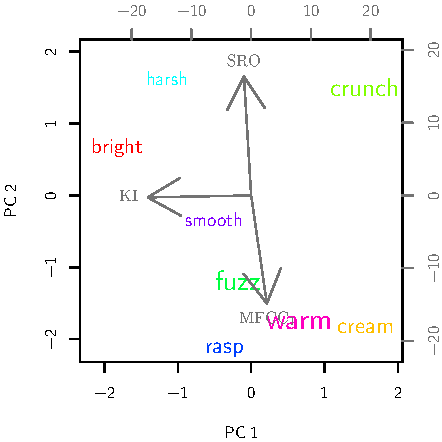
\includegraphics{chapter4/Images/DistortionProcessedCentroidsPCA1-2.pdf}
					\label{fig:DistortionProcessedCentroidsPCA1-2}
				}
				\quad
				\subfloat
				{
					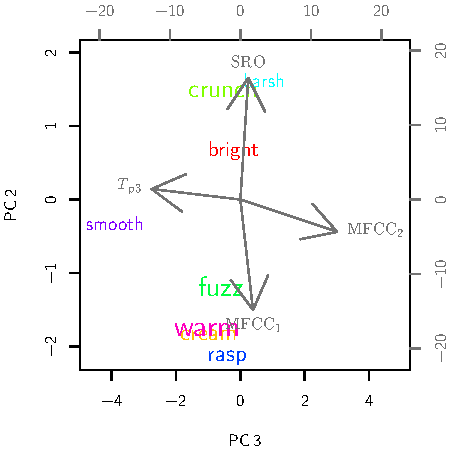
\includegraphics{chapter4/Images/DistortionProcessedCentroidsPCA3-2.pdf}
					\label{fig:DistortionProcessedCentroidsPCA3-2}
				}
				\caption{Biplots of the distortion's processed feature timbre space.}
				\label{fig:DistortionProcessedCentroidsPCAs}
			\end{figure}

			From the analysis of Figure \ref{fig:DistortionProcessedPCAs}, the PCs which best describe each
			term were identified. This information can be used to assist in the analysis of Figure
			\ref{fig:DistortionProcessedCentroidsPCAs}. For instance, while the mean position of signals
			described with the term `crunch' appears to sit at the top end of PC 2, it is known that this
			descriptor's position in PC 2 is not significant.

			Combining the information from both visualisations of the timbre space, it is suggested that the
			terms `warm', `fuzz' and `cream' are characterised by a relatively low spectral roll off, spectral
			standard deviation and spectral centroid. These features describe low bandwidth signals in which
			the energy is concentrated in the low end of the spectrum. `Crunchiness' however, is characterised
			by a relatively low value of Krimphoff irregularity, spectral kurtosis and spectral skewness,
			indicating a signal in which the energy is more evenly spread throughout the spectrum.

			Looking at the mean bark band spectra for the descriptors (Figure
			\ref{fig:DistortionProcessedSpectra}, the spectral effects of a descriptor's position in PC 2 can
			be seen. As the value of PC 2 increases so does the signals proportion of high frequency content,
			`rasp' and `cream' describing signals will a low proportion of high frequency energy and `bright'
			and `harsh' describing those with a larger proportion. The spectral effects of the other PCs ore
			not as apparent, this is likely due to the low resolution of the spectral representation but could
			also be caused by the low number of instances of some terms.

			\begin{figure}[h!]
				\centering
				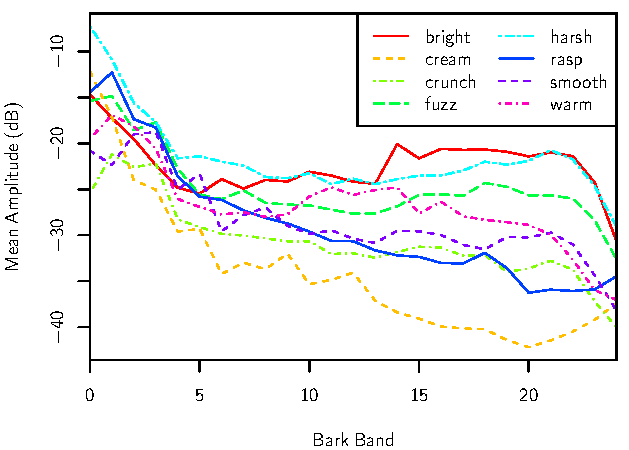
\includegraphics{chapter4/Images/DistortionProcessedSpectra.pdf}
				\caption{The mean bark band spectra of signals produced by the distortion.}
				\label{fig:DistortionProcessedSpectra}
			\end{figure}

		\subsubsection*{Distortion Feature Differences}
			The first three PCs of the timbre space describing the feature manipulations applied by the
			distortion are shown in Figure \ref{fig:DistortionDifferencePCAs}. The corresponding agreement
			scores are shown in Table \ref{tab:DistortionDifferenceAgreements}. This space is largely similar
			to that describing the distortion's processed signals (Figure \ref{fig:DistortionProcessedPCAs})
			and similar conclusions can be drawn.

			\begin{figure}[h!]
				\centering
				\subfloat
				{
					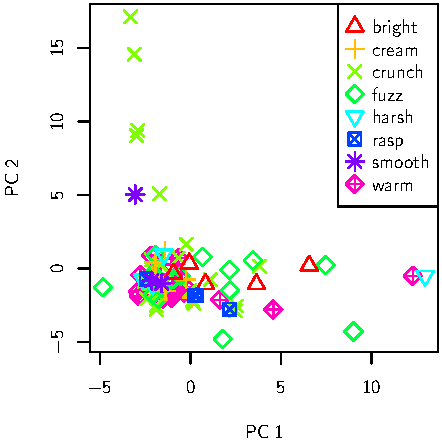
\includegraphics{chapter4/Images/DistortionDifferencePCA1-2.pdf}
					\label{fig:DistortionDifferencePCA1-2}
				}
				\quad
				\subfloat
				{
					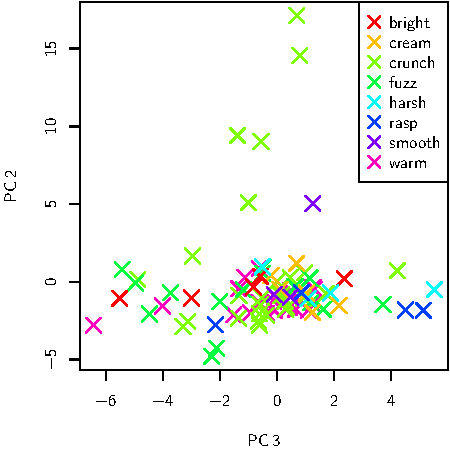
\includegraphics{chapter4/Images/DistortionDifferencePCA3-2.pdf}
					\label{fig:DistortionDifferencePCA3-2}
				}
				\caption{The distortion's feature difference timbre space.}
				\label{fig:DistortionDifferencePCAs}
			\end{figure}

			\begin{table}[h!]
				\centering
				\begin{tabular}{|c|c|}
	\hline
	\bf{Term} & \bf{Agreement} \tabularnewline
	\hline
	\hline
	warm & 0.7 \tabularnewline
	\hline
	crunch & 0.6 \tabularnewline
	\hline
	cream & 0.6 \tabularnewline
	\hline
	fuzz & 0.5 \tabularnewline
	\hline
\end{tabular}
\qquad
\begin{tabular}{|c|c|}
	\hline
	\bf{Term} & \bf{Agreement} \tabularnewline
	\hline
	\hline
	rasp & 0.3 \tabularnewline
	\hline
	bright & 0.2 \tabularnewline
	\hline
	harsh & 0.2 \tabularnewline
	\hline
	smooth & 0.1 \tabularnewline
	\hline
\end{tabular}

				\centering
				\caption{The agreement scores for terms in the 
					 distortion's feature difference timbre space.}
				\label{tab:DistortionDifferenceAgreements}
			\end{table}

			Again `warm', `fuzz' and `cream' are best defined by their position in PC 1 while crunch is better
			defined in PC 2. For the majority of the descriptors the agreement scores are not substantially
			different from those calculated in the processed feature timbre space, making it uncertain whether
			the terms best describe a signal's features or the manipulations applied by a transform. `cream'
			does receive a higher agreement score but the small number of transforms labelled with this
			descriptor (6) reduces the significance of any conclusions drawn from this.

			The salient features for this timbre space are shown in Datum
			\ref{dat:DistortionDifferenceCorrelations}. The most salient in each PC are then visualised, along
			with the mean position and agreement score of each descriptor, in Figure
			\ref{fig:DistortionDifferenceCentroidsPCAs}. 

			\begin{datum}[h!]
				\centering
				\begin{minipage}{0.9\textwidth}
					{\bf{PC 1:}} $\textrm{KI}$~($r~=~{0.992}$), $\textrm{KI}_{\textrm{p}}$~($r~=~{0.989}$), $\textrm{KI}_{\textrm{h}}$~($r~=~{0.971}$), $\gamma_{\textrm{p}}$~($r~=~{0.956}$), $\kappa_{\textrm{p}}$~($r~=~{0.956}$), $\gamma_{\textrm{h}}$~($r~=~{0.943}$), $\kappa_{\textrm{h}}$~($r~=~{0.941}$), $\sigma$~($r~=~{0.939}$), $\textrm{RMS}$~($r~=~{0.939}$), $\gamma_{\textrm{s}}$~($r~=~{0.918}$), $\sigma^{2}$~($r~=~{0.877}$), $\kappa_{\textrm{s}}$~($r~=~{0.744}$).\vspace{0.5em}\\
{\bf{PC 2:}} $\textrm{SRO}$~($r~=~{-0.913}$), $\mu_{\textrm{s}}$~($r~=~{-0.901}$), $\sigma_{\textrm{h}}$~($r~=~{-0.869}$), $\mu_{\textrm{h}}$~($r~=~{-0.832}$), $\sigma_{\textrm{p}}$~($r~=~{-0.831}$), $\mu_{\textrm{p}}$~($r~=~{-0.830}$), $\textrm{SSl}$~($r~=~{-0.793}$), $\sigma_{\textrm{s}}^{2}$~($r~=~{-0.764}$), $\sigma_{\textrm{s}}$~($r~=~{-0.761}$), $\sigma_{\textrm{p}}^{2}$~($r~=~{-0.725}$), $\sigma_{\textrm{h}}^{2}$~($r~=~{-0.719}$), $\textrm{ZCR}$~($r~=~{-0.715}$).\vspace{0.5em}\\
{\bf{PC 3:}} $T_{1}$~($r~=~{-0.797}$), $T_{\textrm{p}1}$~($r~=~{-0.783}$).

				\end{minipage}
				\caption{The salient features of the distortion's
					 feature difference timbre space.}
				\label{dat:DistortionDifferenceCorrelations}
			\end{datum}

			\begin{figure}[h!]
				\centering
				\subfloat
				{
					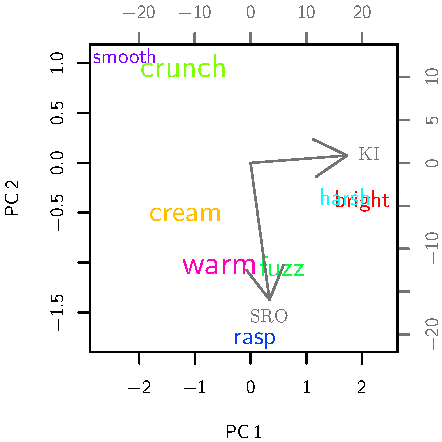
\includegraphics{chapter4/Images/DistortionDifferenceCentroidsPCA1-2.pdf}
					\label{fig:DistortionDifferenceCentroidsPCA1-2}
				}
				\quad
				\subfloat
				{
					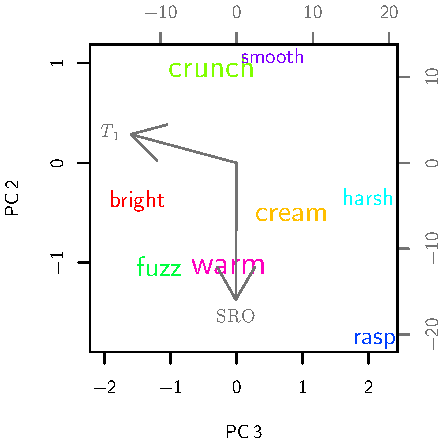
\includegraphics{chapter4/Images/DistortionDifferenceCentroidsPCA3-2.pdf}
					\label{fig:DistortionDifferenceCentroidsPCA3-2}
				}
				\caption{Biplots of the distortion's feature difference timbre space.}
				\label{fig:DistortionDifferenceCentroidsPCAs}
			\end{figure}

			PC 2 is again correlated with spectral roll off, spectral centroid and spectral standard deviation.
			Referring to the raw values of the feature differences, there is no definite direction in which
			these features and moved by the transforms labelled with `warm', `fuzz' and `crunch'. This is
			reflected in Figure \ref{fig:DistortionProcessedSpectra} where the mean spectral manipulations for
			these descriptors are mostly flat. This is an indication that, when used for describing signals
			processed by distortion, these descriptors describe features of the output signal rather than of
			the transform applied.

			PC 1 is correlated with Krimphoff irregularity, spectral skewness and spectral kurtosis, the
			position of `crunch' in this PC corresponding to a small increase in each of these features.
			Looking at the bark band spectra and spectral manipulations in Figures
			\ref{fig:DistortionProcessedSpectra} and \ref{fig:DistortionDifferenceSpectra} the magnitude of
			these increases can be investigated. For `crunch', at the low end of PC 1, a small amount higher
			frequency energy is introduced creating a signal in which the energy is more evenly distributed
			throughout the spectrum. For `bright', at the other end of PC 1, much larger amounts of high
			frequency energy is added, producing signals in which there is more energy at high frequencies than
			at mid frequencies.

			\begin{figure}[h!]
				\centering
				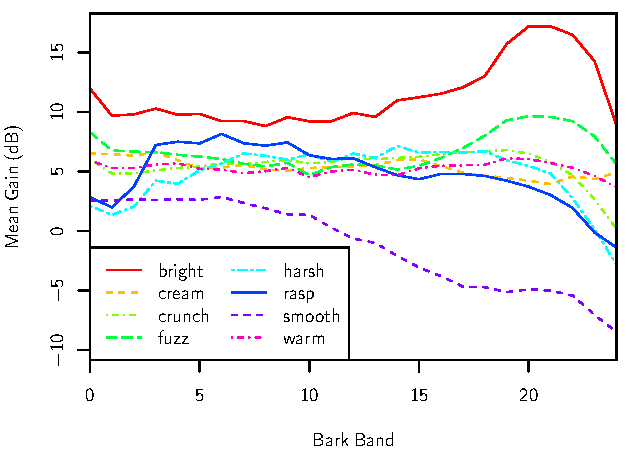
\includegraphics{chapter4/Images/DistortionDifferenceSpectra.pdf}
				\caption{The mean spectral manipulations applied using the distortion.}
				\label{fig:DistortionDifferenceSpectra}
			\end{figure}

		\subsubsection*{Equaliser Processed Features}
			To avoid the large number of instances of the terms `warm' and `bright' from obscuring the other
			terms, the equaliser timbre spaces have been split across two sets of graphs. One showing the
			positions of `warm' and `bright' and the other showing the positions of the remaining descriptors.
			The first three PCs of the timbre space describing the processed signals produced by the equaliser
			are shown in Figures \ref{fig:EqualiserBWProcessedPCAs} and \ref{fig:EqualiserProcessedPCAs}. The
			corresponding agreement scores are shown in Table \ref{tab:EqualiserProcessedAgreements}.

			\begin{figure}[h!]
				\centering
				\subfloat
				{
					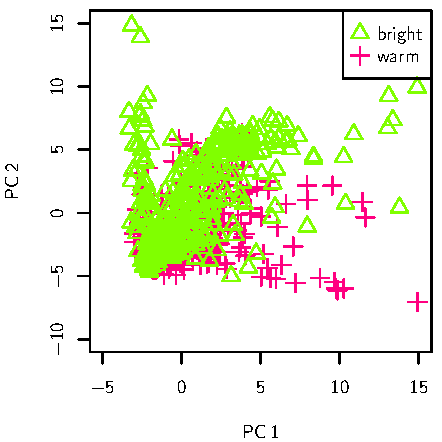
\includegraphics{chapter4/Images/EqualiserBWProcessedPCA1-2.pdf}
					\label{fig:EqualiserProcessedPCA1-2}
				}
				\quad
				\subfloat
				{
					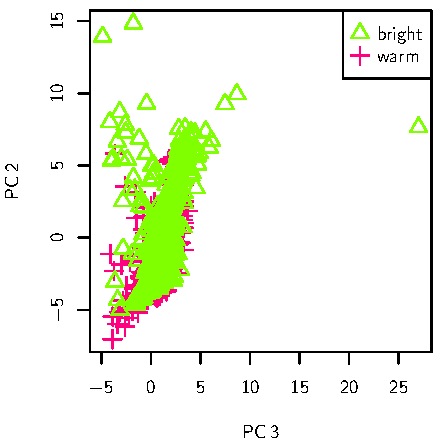
\includegraphics{chapter4/Images/EqualiserBWProcessedPCA3-2.pdf}
					\label{fig:EqualiserProcessedPCA3-2}
				}
				\caption{Signals labelled with `warm' and `bright' in the equaliser's processed
					 feature timbre space.}
				\label{fig:EqualiserBWProcessedPCAs}
			\end{figure}

			\begin{figure}[h!]
				\centering
				\subfloat
				{
					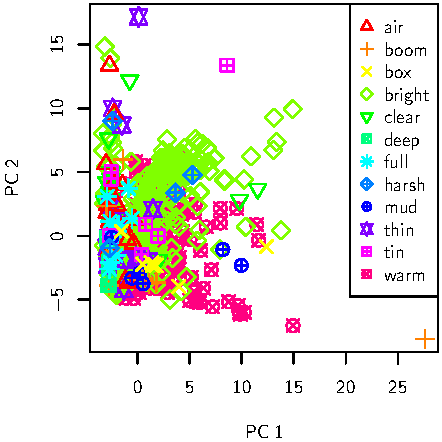
\includegraphics{chapter4/Images/EqualiserProcessedPCA1-2.pdf}
					\label{fig:EqualiserProcessedPCA1-2}
				}
				\quad
				\subfloat
				{
					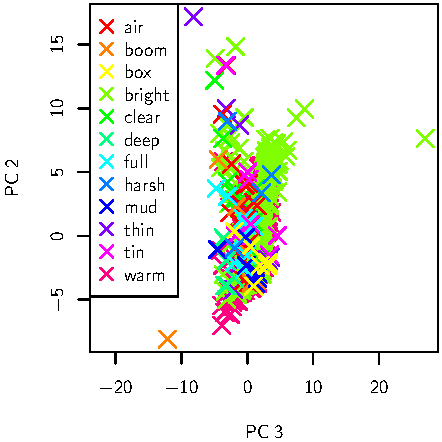
\includegraphics{chapter4/Images/EqualiserProcessedPCA3-2.pdf}
					\label{fig:EqualiserProcessedPCA3-2}
				}
				\caption{The remainder of the equaliser's processed feature timbre space.}
				\label{fig:EqualiserProcessedPCAs}
			\end{figure}

			\begin{table}[h!]
				\centering
				\begin{tabular}{|c|c|}
	\hline
	\bf{Term} & \bf{Agreement} \tabularnewline
	\hline
	\hline
	warm & 1.53 \tabularnewline
	\hline
	bright & 1.24 \tabularnewline
	\hline
	deep & 0.95 \tabularnewline
	\hline
	air & 0.64 \tabularnewline
	\hline
\end{tabular}
\qquad
\begin{tabular}{|c|c|}
	\hline
	\bf{Term} & \bf{Agreement} \tabularnewline
	\hline
	\hline
	box & 0.59 \tabularnewline
	\hline
	mud & 0.58 \tabularnewline
	\hline
	full & 0.54 \tabularnewline
	\hline
	thin & 0.52 \tabularnewline
	\hline
\end{tabular}
\qquad
\begin{tabular}{|c|c|}
	\hline
	\bf{Term} & \bf{Agreement} \tabularnewline
	\hline
	\hline
	clear & 0.48 \tabularnewline
	\hline
	boom & 0.47 \tabularnewline
	\hline
	tin & 0.42 \tabularnewline
	\hline
	harsh & 0.08 \tabularnewline
	\hline
\end{tabular}

				\caption{The agreement scores for terms in the 
					 equaliser's processed feature timbre space.}
				\label{tab:EqualiserProcessedAgreements}
			\end{table}

			Within the equaliser's processed feature timbre space, the terms `warm' and `bright' do not occupy
			distinct regions to one another. This reflects the clustering of these terms seen in Figure
			\ref{fig:EqualiserProcessedClusters}, again suggesting that these terms have not been used to
			describe distinct properties of the processed signal. The remaining descriptors are also difficult
			to distinguish. One apparent pattern is the separation of `harsh' and `mud' in PC 2, although this
			may be due to chance as the agreement score for `harsh' is very low.

			The salient features for this timbre space are shown in Datum
			\ref{dat:EqualiserProcessedCorrelations}. The most salient in each PC are then visualised, along
			with the mean position and agreement score of each descriptor, in Figure
			\ref{fig:EqualiserProcessedCentroidsPCAs}. These show that, although the clusters for each term are
			not well separated, their centroids are positioned in the timbre space as one might expect.

			\begin{datum}[h!]
				\centering
				\begin{minipage}{0.9\textwidth}
					{\bf{PC 1:}} $\mathrm{KI}$~($r~=~{0.991}$), $\mathrm{KI_{p}}$~($r~=~{0.981}$), $\kappa_{\mathrm{h}}$~($r~=~{0.966}$), $\kappa_{\mathrm{p}}$~($r~=~{0.962}$), $\mathrm{KI_{h}}$~($r~=~{0.958}$), $\gamma_{\mathrm{s}}$~($r~=~{0.945}$), $\gamma_{\mathrm{p}}$~($r~=~{0.895}$), $\gamma_{\mathrm{h}}$~($r~=~{0.886}$), $\kappa_{\mathrm{s}}$~($r~=~{0.884}$), $\sigma$~($r~=~{0.840}$), $\mathrm{RMS}$~($r~=~{0.840}$), $\sigma^{2}$~($r~=~{0.813}$).\vspace{0.5em}\\
{\bf{PC 2:}} $\sigma_{\mathrm{h}}$~($r~=~{ 0.922}$), $\sigma_{\mathrm{p}}$~($r~=~{ 0.918}$), $\mathrm{SRO}$~($r~=~{ 0.895}$), $\mu_{\mathrm{h}}$~($r~=~{ 0.881}$), $\mu_{\mathrm{p}}$~($r~=~{ 0.881}$), $\mu_{\mathrm{s}}$~($r~=~{ 0.806}$), $\mathrm{SSl}$~($r~=~{ 0.805}$), $\mathrm{MFCC}_{1}$~($r~=~{-0.802}$), $\mathrm{ZCR}$~($r~=~{ 0.798}$), $\sigma_{\mathrm{p}}^{2}$~($r~=~{ 0.761}$), $\sigma_{\mathrm{h}}^{2}$~($r~=~{ 0.761}$), $T_{\mathrm{p}2}$~($r~=~{-0.749}$), $T_{2}$~($r~=~{-0.745}$), $\mathrm{SC}$~($r~=~{-0.720}$).\vspace{0.5em}\\
{\bf{PC 3:}} $\mathrm{MFCC}_{4}$~($r~=~{-0.718}$), $\mathrm{MFCC}_{2}$~($r~=~{-0.715}$), $\sigma_{\mathrm{s}}$~($r~=~{-0.714}$).\vspace{0.5em}\\
{\bf{PC 4:}} $\mathrm{MFCC}_{8}$~($r~=~{0.926}$), $\mathrm{MFCC}_{10}$~($r~=~{0.839}$), $\mathrm{MFCC}_{9}$~($r~=~{0.836}$), $\mathrm{MFCC}_{12}$~($r~=~{0.760}$), $\mathrm{MFCC}_{7}$~($r~=~{0.725}$), $\mathrm{MFCC}_{11}$~($r~=~{0.721}$).\vspace{0.5em}\\
{\bf{PC 5:}} $\mathrm{MFCC}_{5}$~($r~=~{0.743}$), $\mathrm{MFCC}_{3}$~($r~=~{0.705}$).

				\end{minipage}
				\caption{The salient features of the equaliser's
					 processed feature timbre space.}
				\label{dat:EqualiserProcessedCorrelations}
			\end{datum}

			\begin{figure}[h!]
				\centering
				\subfloat
				{
					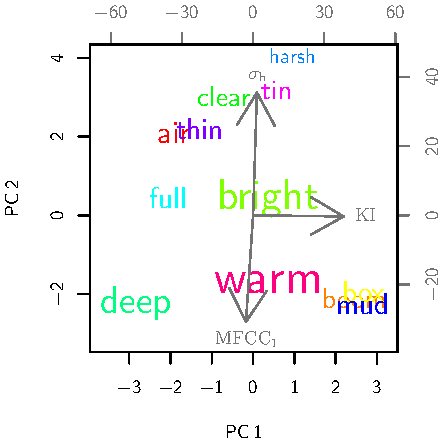
\includegraphics{chapter4/Images/EqualiserProcessedCentroidsPCA1-2.pdf}
					\label{fig:EqualiserProcessedCentroidsPCA1-2}
				}
				\quad
				\subfloat
				{
					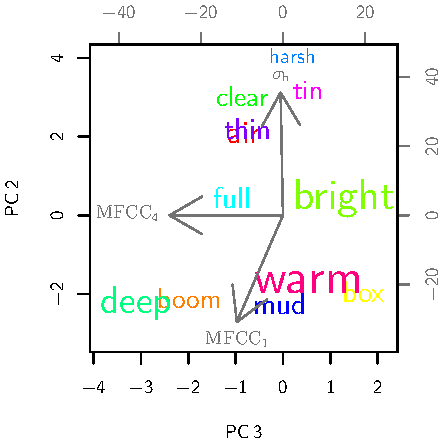
\includegraphics{chapter4/Images/EqualiserProcessedCentroidsPCA3-2.pdf}
					\label{fig:EqualiserProcessedCentroidsPCA3-2}
				}
				\caption{Biplots of the equaliser's processed feature timbre space.}
				\label{fig:EqualiserProcessedCentroidsPCAs}
			\end{figure}

			PC 2 is correlated with spectral standard deviation, spectral roll off and spectral centroid.
			Signals with a larger proportion of high frequency energy being positioned at the top and those
			with more low frequency energy at the bottom. The descriptors are spread out across this dimension,
			illustrating a general trend that `deep', `mud', `boom' and `warm' are used to describe high
			proportions of low frequencies and 'harsh', 'tin' and 'clear' used to describe higher proportions
			of high frequencies. Examining the mean bark band spectra of these signals (Figure
			\ref{fig:EqualiserProcessedSpectra}) these trends can be seen. 

			\begin{figure}[h!]
				\centering
				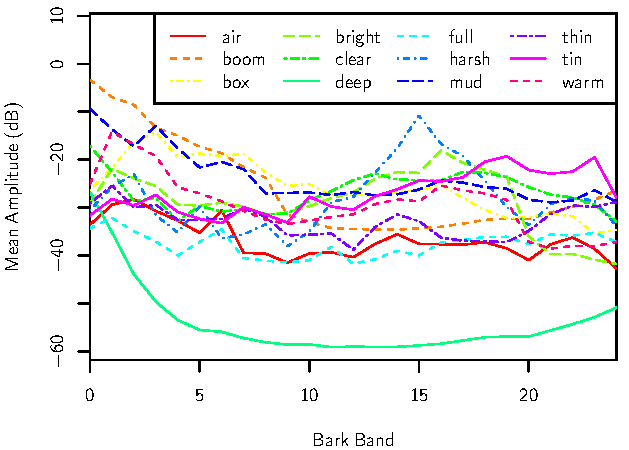
\includegraphics{chapter4/Images/EqualiserProcessedSpectra.pdf}
				\caption{The mean bark band spectra of signals produced by the equaliser.}
				\label{fig:EqualiserProcessedSpectra}
			\end{figure}

			PC 1 seems to separate the low frequency descriptors into groups. `deep' describing signals with
			smoother spectra and a greater skew towards lower frequencies than those described by `boom' and
			`mud'. This difference is apparent in Figure \ref{fig:EqualiserProcessedSpectra}, signals described
			as `deep' containing predominantly low frequency energy and those described as `boom' and `mud'
			having more complex spectra but still with a large proportion of low frequency energy.

		\subsubsection*{Equaliser Feature Differences}
			The first three PCs of the timbre space describing the feature manipulations applied by the
			equaliser are shown in Figures \ref{fig:EqualiserBWDifferencePCAs} and
			\ref{fig:EqualiserDifferencePCAs}. The corresponding agreement scores are shown in Table
			\ref{tab:EqualiserDifferenceAgreements}. This space shows more definite patterns than that
			constructed from the processed feature values.

			\begin{figure}[h!]
				\centering
				\subfloat
				{
					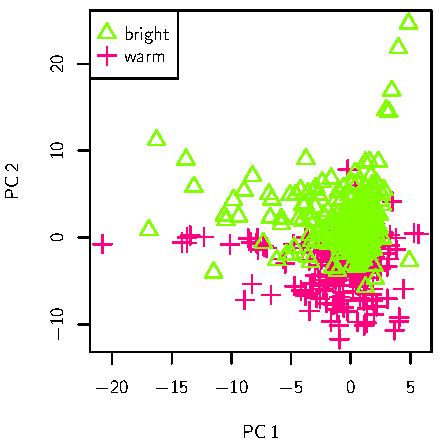
\includegraphics{chapter4/Images/EqualiserBWDifferencePCA1-2.pdf}
					\label{fig:EqualiserDifferencePCA1-2}
				}
				\quad
				\subfloat
				{
					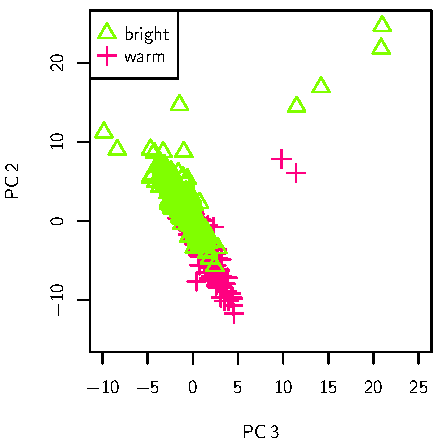
\includegraphics{chapter4/Images/EqualiserBWDifferencePCA3-2.pdf}
					\label{fig:EqualiserDifferencePCA3-2}
				}
				\caption{Transforms labelled with `warm' and `bright' in the equaliser's
					 feature difference timbre space.}
				\label{fig:EqualiserBWDifferencePCAs}
			\end{figure}

			\begin{figure}[h!]
				\centering
				\subfloat
				{
					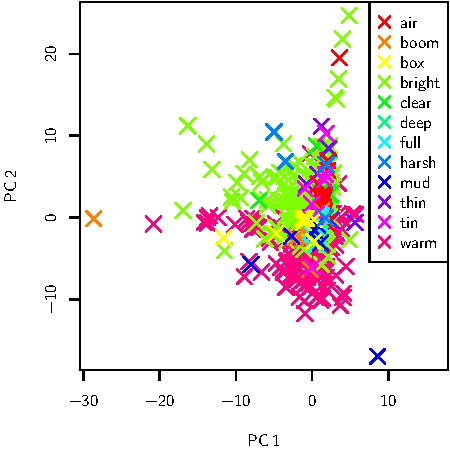
\includegraphics{chapter4/Images/EqualiserDifferencePCA1-2.pdf}
					\label{fig:EqualiserDifferencePCA1-2}
				}
				\quad
				\subfloat
				{
					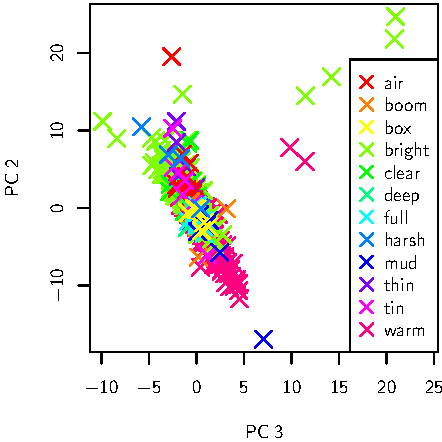
\includegraphics{chapter4/Images/EqualiserDifferencePCA3-2.pdf}
					\label{fig:EqualiserDifferencePCA3-2}
				}
				\caption{The remainder of the equaliser's feature difference timbre space.}
				\label{fig:EqualiserDifferencePCAs}
			\end{figure}

			\begin{table}[h!]
				\centering
				\begin{tabular}{|c|c|}
	\hline
	\bf{Term} & \bf{Agreement} \tabularnewline
	\hline
	\hline
	warm & 1.49 \tabularnewline
	\hline
	bright & 1.19 \tabularnewline
	\hline
	deep & 1.17 \tabularnewline
	\hline
	full & 0.79 \tabularnewline
	\hline
\end{tabular}
\qquad
\begin{tabular}{|c|c|}
	\hline
	\bf{Term} & \bf{Agreement} \tabularnewline
	\hline
	\hline
	air & 0.71 \tabularnewline
	\hline
	box & 0.49 \tabularnewline
	\hline
	clear & 0.45 \tabularnewline
	\hline
	thin & 0.38 \tabularnewline
	\hline
\end{tabular}
\qquad
\begin{tabular}{|c|c|}
	\hline
	\bf{Term} & \bf{Agreement} \tabularnewline
	\hline
	\hline
	mud & 0.33 \tabularnewline
	\hline
	tin & 0.30 \tabularnewline
	\hline
	boom & 0.27 \tabularnewline
	\hline
	harsh & 0.05 \tabularnewline
	\hline
\end{tabular}

				\caption{The agreement scores for terms in the 
					 equaliser's feature difference timbre space.}
				\label{tab:EqualiserDifferenceAgreements}
			\end{table}

			The clusters of transforms labelled with `warm' and `bright' are now better separated in PC 2,
			`bright' taking positive values and `warm' negative values. In the other PCs these descriptors
			occupy very similar ranges, suggesting that the distinction between these descriptors is in how the
			features which correlate with PC 2 are manipulated. The clusters of the remaining descriptors are
			again difficult to discriminate, the separation of `harsh' and `mud' in PC 2 being the most
			noticeable pattern.

			The salient features for this timbre space are shown in Datum
			\ref{dat:EqualiserDifferenceCorrelations}. The most salient in each PC are then visualised, along
			with the mean position and agreement score of each descriptor, in Figure
			\ref{fig:EqualiserDifferenceCentroidsPCAs}. 

			\begin{datum}[h!]
				\centering
				\begin{minipage}{0.9\textwidth}
					\begin{itemize}
	\item {\bf{PC 1:}} $\textrm{KI}$~($r~=~-0.986$), $\textrm{KI}_{\textrm{p}}$~($r~=~-0.970$), $\gamma_{\textrm{s}}$~($r~=~-0.968$), $\kappa_{\textrm{p}}$~($r~=~-0.932$), $\textrm{KI}_{\textrm{h}}$~($r~=~-0.922$), $\kappa_{\textrm{s}}$~($r~=~-0.915$), $\kappa_{\textrm{h}}$~($r~=~-0.912$), $\sigma^{2}$~($r~=~-0.890$), $\sigma$~($r~=~-0.872$), $\textrm{RMS}$~($r~=~-0.872$), $\gamma_{\textrm{p}}$~($r~=~-0.862$), $\gamma_{\textrm{h}}$~($r~=~-0.831$).
	\item {\bf{PC 2:}} $\mu_{\textrm{p}}$~($r~=~ 0.867$), $\mu_{\textrm{h}}$~($r~=~ 0.863$), $\sigma_{\textrm{h}}$~($r~=~ 0.838$), $\sigma_{\textrm{p}}$~($r~=~ 0.833$), $\textrm{SRO}$~($r~=~ 0.813$), $\mu_{\textrm{s}}$~($r~=~ 0.770$), $\textrm{SSl}$~($r~=~ 0.745$), $\textrm{MFCC}_{1}$~($r~=~-0.705$).
	\item {\bf{PC 3:}} $\textrm{MFCC}_{5}$~($r~=~-0.794$), $\textrm{MFCC}_{6}$~($r~=~-0.791$), $\textrm{MFCC}_{7}$~($r~=~-0.741$), $\textrm{MFCC}_{0}$~($r~=~ 0.723$), $\textrm{JI}$~($r~=~ 0.722$).
	\item {\bf{PC 4:}} $\textrm{MFCC}_{12}$~($r~=~0.917$), $\textrm{MFCC}_{11}$~($r~=~0.908$), $\textrm{MFCC}_{10}$~($r~=~0.893$), $\textrm{MFCC}_{9}$~($r~=~0.848$), $\textrm{MFCC}_{8}$~($r~=~0.742$).
\end{itemize}

				\end{minipage}
				\caption{The salient features of the equaliser's
					 feature difference timbre space.}
				\label{dat:EqualiserDifferenceCorrelations}
			\end{datum}

			\begin{figure}[h!]
				\centering
				\subfloat
				{
					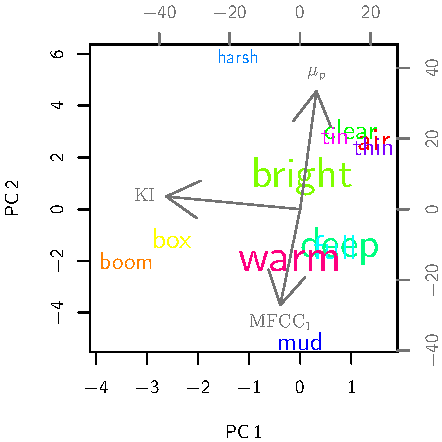
\includegraphics{chapter4/Images/EqualiserDifferenceCentroidsPCA1-2.pdf}
					\label{fig:EqualiserDifferenceCentroidsPCA1-2}
				}
				\quad
				\subfloat
				{
					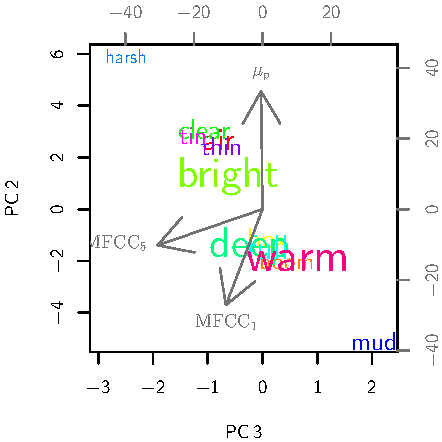
\includegraphics{chapter4/Images/EqualiserDifferenceCentroidsPCA3-2.pdf}
					\label{fig:EqualiserDifferenceCentroidsPCA3-2}
				}
				\caption{Biplots of the equaliser's feature difference timbre space.}
				\label{fig:EqualiserDifferenceCentroidsPCAs}
			\end{figure}

			The distinction between `warm' and `bright' becomes very clear here. PC 2 is highly correlated with
			spectral centroid, spectral standard deviation and spectral roll off. Negative values of PC 2
			correspond to a decrease in these features and positive values an increase. Signals can be made
			`warmer' by reducing the spectral centroid and `brighter' by increasing it. This is most often done
			by introducing more energy at low or higher frequencies respectively, as seen in Figure
			\ref{fig:EqualiserDifferenceSpectra}. `harsh' and `tin' can be thought of as more accentuated
			versions of `bright' and `mud' as a more accentuated version of `warm'.

			The more distinct patterns seen by using the feature differences suggest that these terms have been
			used to describe the transform rather than he output signal. The process of making a signal
			`warmer' or `brighter' is independent of the absolute value of spectral centroid or spectral roll
			off. It is the direction in which these features are moved which is being described. This makes it
			conceptually easier to control audio in terms of these descriptors, rather than producing an output
			with a particular feature value, the feature need only be moved in the correct direction.

			\begin{figure}[h!]
				\centering
				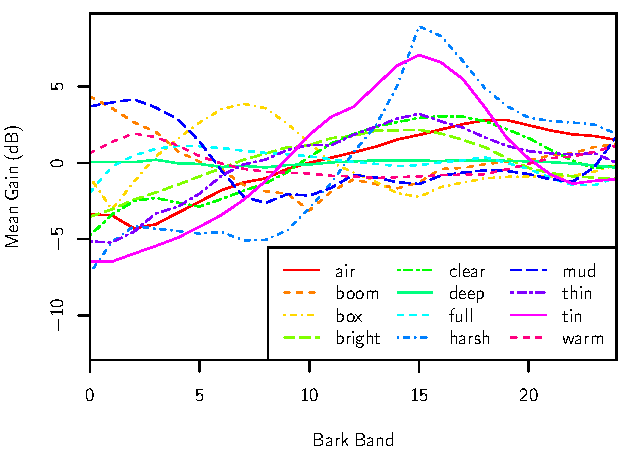
\includegraphics{chapter4/Images/EqualiserDifferenceSpectra.pdf}
				\caption{The mean spectral manipulations applied using the equaliser.}
				\label{fig:EqualiserDifferenceSpectra}
			\end{figure}

			The usage of `deep' in the dataset seems to be a property of the input signals being used. Figure
			\ref{fig:EqualiserDifferenceSpectra} shows that very little manipulation was applied in producing a
			`deep' signal. While it is clear from Figure \ref{fig:EqualiserProcessedSpectra} that `deep'
			describes signals with a large proportion of low frequency energy, no processing has been applied
			to cause this. As such, the signals must have been `deep' prior to processing.

\section{Results Summary}
	\note
	{
		Summarise those results!

		\begin{itemize}
			\item Four main groups of descriptors, `warm', `bright', `crunch' and `mud'.
			\item `warm' is used similarly across both plug-ins.
			\item `bright' seems to mean slightly different things depending on the processing, this could be
				due to the way each system adds high frequency energy. Distortion `bright' is synonymous
				with `harsh'. While equaliser `bright' and `harsh' are more distinct.
			\item `warm' is associated with spectral centroid, spectral roll off and spectral standard
				deviation. With distortion like effects it describes output signals which have more low
				frequencies than high. With eq like effects it describes transforms which skew the spectrum
				towards the lower end.
			\item `bright' is associated with the same features but at the other extreme, greater proportions
				of high frequency energy. In the eq `harsh' is a more pronounced version of it, whereas in
				the distortion `harsh' is synonymous.
			\item `crunchiness' is a descriptor associated with distortion only. It describes distortion which
				flattens out the spectrum, not introducing too much high frequency energy to become
				`harsh'.
			\item `mud' is associated with high levels of low frequency energy, a more accentuated version of
				`warm'.
		\end{itemize}
	}
